%!TEX root = ../thesis.tex
% TODO: Change this?

\chapter{Immunoglobulin sequencing in \textit{Nothobranchius furzeri}} 
\label{chap:igseq}
 
\onehalfspacing

% Chapter summary (should fit on title page)
\section*{Summary} 

\dots
\pagebreak

% Sections

\section{Introduction}

%To understand and counter the complex changes that occur in the adaptive immune system with age, it is necessary to analyse the whole population of lymphocyte antigen-receptor sequences present in an individual. Such a top-down approach was impossible until relatively recently, when the advent of modern high-throughput sequencing technologies enabled the development of specialised protocols for immune-repertoire sequencing and analysis. Since then, the field of immune-repertoire studies has developed rapidly, providing a new and more powerful method for interrogating the changes ocurring in adaptive immune repertoires in a wide variety of contexts, including ageing. However, while initial human studies have indicated a decline in the diversity of these repertoires in older people, there remains a need for further research in this area. % This is weak, fill in once you've done your lit review.

%\section{Quantifying antibody repertoire composition with immunoglobulin sequencing}
%\label{sec:intro_igseq}
%
%% TODO: Move these paragraphs to IgSeq chapter intro?
%
%As a result of the primary and secondary diversification mechanisms described in \Cref{sec:intro_immunity_primary,sec:intro_affinity_maturation}, the population of B-cells present in the body of a mature jawed vertebrate together express an enormous diversity of unique antibody sequences, with a correspondingly vast array of antigen specificities.  This huge population of sequences contains a considerable amount of structure: \naive sequences in the primary repertoire are produced by the same underlying generative and selective process and so share common statistical properties, while many sequences in the secondary repertoire are related to one another as members of clones descended from a common \naive B-cell ancestor. By sampling the repertoire of antibody sequences present in a sample and reconstructing its underlying recombinatorial and clonal structure, much can be learned about the history and current state of humoral adaptive immununity in that organism.
%
%The advent of modern high-throughput sequencing mechanisms enabled the development of specialised sequencing techniques designed to interrogate the antibody repertoire, via targeted sequencing of B-cell DNA or RNA. From the beginning, these \Igseq (or \igseq) studies included teleost model organisms, with early \igseq studies investigating the antibody repertoire of developing and adult zebrafish. These studies revealed ... % Describe results from early zebrafish studies

%Caruso \textit{et al.} \parencite{caruso2009immunosenescence} commented that, though the antibody repertoire diversity of mucosal systems had not (and, to my knowledge, has still not) been investigated specifically, the fact that these regions undergo especially frequent antigenic challenge and consequent clonal expansion of antigen-experienced cells suggests that they might be expected to show a particularly strong decline in repertoire diversity with age, impairing the ability of the organism to regulate its mucosal microbiotal environments...

% TODO: Move to discussion chapter?
% Conversely, the most well-developed teleost model organism, the zebrafish, is relatively distantly-related, with an estimated divergence time of over 200 Mya \parencite{hughes2018teleostphylo}, making the use in a killifish context of the many genetic and experimental resources developed for the zebrafish more challenging. As a result, techniques such as cell-type-specific cell sorting that depend on cell-surface markers or specific antibodies are currently unavailable for killifish studies, though many are under active development in one or more killifish laboratories.

%Turquoise killifish are strongly sexually dimorphic, with an XY sex-determination system \parencite{reichwald2015genome,valenzano2009map} and large, colourful males. Most killifish studies to date have been performed using fish of only one sex, typically males; this thesis is no exception.


\dots

\section{Collecting killifish samples for immunoglobulin sequencing}
\label{sec:igseq_samples}

To obtain samples for establishing and validating an \Igseq protocol in turquoise killifish, as well as to investigate changes in killifish repertoires with age, male GRZ-AD turquoise killifish from a single hatching cohort were raised under standard husbandry conditions (\Cref{sec:methods_husbandry}) and sacrificed by anaesthesia, followed by flash-freezing in liquid nitrogen and preservation at \degC{-80}. In total, thirty-two fish were sacrificed at four total time points (\Cref{tab:igseq-cohorts-summary,tab:igseq-cohorts-fish}): regular groups of ten fish each were sacrificed at roughly 5.5 weeks (shortly after reproductive maturation), 8 weeks (middle adulthood) and 10.5 weeks (close to median lifespan) post-hatching, while two surviving fish were sacrificed eight weeks later at roughly 18 weeks post-hatching.

\begin{table}
\caption{Summary of killifish used in \igseq validation and ageing experiment. All fish are GRZ-AD strain and male.}
\label{tab:igseq-cohorts-summary}
% latex table generated in R 3.5.2 by xtable 1.8-3 package
% Wed Jan 30 11:19:43 2019
\begin{tabular}{rrlllll}
  \toprule Group & \# Fish & Hatch date & Sacrifice date & Age (days) & Age (weeks) & Mean weight (g) \\ 
  \midrule 1 & 10 & 2016-05-09 & 2016-06-17 & 39 & 5.57 & 1.3 \\ 
  2 & 10 & 2016-05-09 & 2016-07-04 & 56 & 8 & 1.37 \\ 
  3 & 10 & 2016-05-09 & 2016-07-21 & 73 & 10.4 & 1.76 \\ 
  4 & 2 & 2016-05-09 & 2016-09-14 & 128 & 18.3 & 2.3 \\ 
   \bottomrule \end{tabular}

\end{table}

\begin{table}
\caption{Turquoise killifish used in \igseq validation and ageing experiment. All fish are GRZ-AD strain and male.}
\label{tab:igseq-cohorts-fish}
\begin{threeparttable}
% latex table generated in R 3.5.2 by xtable 1.8-3 package
% Wed Jan 30 11:19:43 2019
\begin{tabular}{rrrrllrr}
  \toprule Group & \# & Fish ID\tnote{1} & Death weight (g) & Hatch date & Sacrifice date & Age (days) & Age (weeks) \\ 
  \midrule 1 & 1 & 4194 & 1.24 & 2016-05-09 & 2016-06-17 &  39 &  5.57 \\ 
  1 & 2 & 4107 & 1.39 & 2016-05-09 & 2016-06-17 &  39 &  5.57 \\ 
  1 & 3 & 4127 & 1.29 & 2016-05-09 & 2016-06-17 &  39 &  5.57 \\ 
  1 & 4 & 4204 & 1.35 & 2016-05-09 & 2016-06-17 &  39 &  5.57 \\ 
  1 & 5 & 4189 & 1.43 & 2016-05-09 & 2016-06-17 &  39 &  5.57 \\ 
  1 & 6 & 4160 & 0.68 & 2016-05-09 & 2016-06-17 &  39 &  5.57 \\ 
  1 & 7 & 4164 & 1.57 & 2016-05-09 & 2016-06-17 &  39 &  5.57 \\ 
  1 & 8 & 4171 & 1.40 & 2016-05-09 & 2016-06-17 &  39 &  5.57 \\ 
  1 & 9 & 4200 & 1.42 & 2016-05-09 & 2016-06-17 &  39 &  5.57 \\ 
  1 & 10 & 4131 & 1.27 & 2016-05-09 & 2016-06-17 &  39 &  5.57 \\\midrule
  2 & 1 & 4159 & 1.37 & 2016-05-09 & 2016-07-04 &  56 &  8.00 \\ 
  2 & 2 & 4179 & 1.47 & 2016-05-09 & 2016-07-04 &  56 &  8.00 \\ 
  2 & 3 & 4152 & 1.33 & 2016-05-09 & 2016-07-04 &  56 &  8.00 \\ 
  2 & 4 & 4132 & 1.35 & 2016-05-09 & 2016-07-04 &  56 &  8.00 \\ 
  2 & 5 & 4177 & 1.22 & 2016-05-09 & 2016-07-04 &  56 &  8.00 \\ 
  2 & 6 & 4158 & 1.51 & 2016-05-09 & 2016-07-04 &  56 &  8.00 \\ 
  2 & 7 & 4182 & 1.12 & 2016-05-09 & 2016-07-04 &  56 &  8.00 \\ 
  2 & 8 & 4202 & 1.54 & 2016-05-09 & 2016-07-04 &  56 &  8.00 \\ 
  2 & 9 & 4143 & 1.28 & 2016-05-09 & 2016-07-04 &  56 &  8.00 \\ 
  2 & 10 & 4201 & 1.55 & 2016-05-09 & 2016-07-04 &  56 &  8.00 \\\midrule
  3 & 1 & 4155 & 2.06 & 2016-05-09 & 2016-07-21 &  73 & 10.43 \\ 
  3 & 2 & 4193 & 1.92 & 2016-05-09 & 2016-07-21 &  73 & 10.43 \\ 
  3 & 3 & 4170 & 1.80 & 2016-05-09 & 2016-07-21 &  73 & 10.43 \\ 
  3 & 4 & 4135 & 1.65 & 2016-05-09 & 2016-07-21 &  73 & 10.43 \\ 
  3 & 5 & 4190 & 1.87 & 2016-05-09 & 2016-07-21 &  73 & 10.43 \\ 
  3 & 6 & 4099 & 1.94 & 2016-05-09 & 2016-07-21 &  73 & 10.43 \\ 
  3 & 7 & 4198 & 1.49 & 2016-05-09 & 2016-07-21 &  73 & 10.43 \\ 
  3 & 8 & 4024 & 1.73 & 2016-05-09 & 2016-07-21 &  73 & 10.43 \\ 
  3 & 9 & 4044 & 1.53 & 2016-05-09 & 2016-07-21 &  73 & 10.43 \\ 
  3 & 10 & 4117 & 1.57 & 2016-05-09 & 2016-07-21 &  73 & 10.43 \\\midrule
  4 & 1 & 4173 & 2.20 & 2016-05-09 & 2016-09-14 & 128 & 18.29 \\ 
  4 & 2 & 4197 & 2.40 & 2016-05-09 & 2016-09-14 & 128 & 18.29 \\ 
   \bottomrule \end{tabular}

\begin{tablenotes}
\item[1] grz-AD\_...\_E
\end{tablenotes}
\end{threeparttable}
\end{table}

In order to obtain a representative sample of the whole-body antibody repertoires from these individuals (as opposed to the specific repertoire of a particular organ), the frozen fish were homogenised in liquid nitrogen with a mortar and pestle, and total RNA was isolated from the resulting powder with guanidinium thiocyanate-phenol-chloroform extraction (\Cref{sec:methods_molec_standard_qiazol}).

\section{\igseq in the turquoise killifish: principles and protocols}
\label{sec:igseq_protocol}

\subsection{Preparing the \igseq library}
\label{sec:igseq_protocol_library}

\IGSEQ is a precise and quantitative method which is highly sensitive to biases and errors arising during both library preparation (especially PCR) and sequencing. In order to minimise the impact of these errors on the results, unique molecular identifiers (UMIs) are widely used in \igseq library-preparation protocols to uniquely label each input molecule, enabling sequences in the dataset arising from the same input molecule to be identified, grouped and collapsed into a single consensus sequence. This process effectively corrects for biases in apparent abundance arising from differential amplification during library-preparation or differential clustering during sequencing, and allows identical sequences descended from the same input molecule to be distinguished from those descended from different input molecules with the same sequence. In addition, as long as enough reads arising from a given input sequence are present, the taking of a consensus sequence from each UMI group effectively corrects for sequence errors arising during library-preparation and sequencing, enabling the original input sequence to be reconstructed much more accurately (\Cref{fig:umi-consensus-schema}).

In the \igseq protocol established here for the turquoise killifish, the addition of UMIs is achieved through the use of a 5'-RACE-like procedure adapted from \parencite{turchaninova2016igprep}. % TODO: Explain RACE acronym and meaning
This procedure takes advantage of the intrinsic terminal transferase activity exhibited by reverse-transcriptase enzymes derived from Moloney Murine Leukemia Virus (MMLV), which includes most commercially-available reverse-transcriptase enzymes. Upon reaching the end of an RNA template, such viruses add a variable number of untemplated deoxyribonucleotides to the 3'-end of the new cDNA molecule, with a strong bias for cytidine residues. If a template-switch adapter (TSA) oligonucleotide ending in riboguanosines is added to the reaction mixture, it will pair with these untemplated terminal cytidines to form a new priming site for the reverse transcriptase. The enzyme will then re-attach to this new priming site and process to the end of the paired oligo, adding the sequence of the TSA to the 3'-end of the cDNA. This procedure, known as template switching (\Cref{fig:template-switch-schema}), enables semi-arbitrary sequences to be prepended to the reverse-transcribed mRNA sequence, including a primer sequence and (in this case) a UMI. % TODO: Citations for terminal transferase activity

\begin{figure}
\centering
\includegraphics[width=0.7\textwidth]{_Figures/png_edited/umi-consensus-schema}
\caption{\textbf{Correcting errors and biases with unique molecular identifiers (UMIs):} In this simplified schematic, three template RNA molecules representing two distinct sequences (red and blue rectangles) are tagged with UMIs (coloured left-hand ends) prior to PCR-based library preparation and sequencing. As a result of differential amplification bias between the sequences, the less-abundant input sequence gives rise to a larger number of sequencing reads; however, by aligning and collapsing matching UMI groups into consensus reads, the original proportions of the sample can be reconstructed. Consensus-read generation also enables the correction of various PCR and sequencing errors (thin red/green bars), the majority of which are present in only a minority of sequence copies within a UMI group; only the dark-blue UMI group, for which only a single sequencing read was obtained, cannot be effectively corrected in this way.}
\label{fig:umi-consensus-schema}
\end{figure}

\begin{figure}
\centering
\includegraphics[width=0.7\textwidth]{_Figures/png_edited/template-switch-labelled}
\vspace{0.5em}
\caption{\textbf{Addition of a known 5'-sequence with template switching:} In this simplified schematic, an MMLV-derived reverse-transcriptase enzyme (blue oval) binds a primed RNA template and processes to the 5-prime end (A), where it deposits additional untemplated cytidine residues at the 3'-end of the CDNA (red bar) using its terminal-transferase activity (B). A template-switch adaptor (TSA) with complementary terminal guanosine residues (blue bar) pairs with these terminal cytidines (C), creating a new double-stranded priming site to which the reverse-transcriptase enzyme can bind (D). Processing of the enzyme to the end of the TSA sequence produces a cDNA molecule with an additional, known 3' sequence (E).}
\label{fig:template-switch-schema}
\end{figure}

In the library-preparation protocol used for \Igseq in the turquoise killifish, therefore, reverse-transcription is performed on total RNA using a gene-specific primer (GSP) homologous to the constant-region sequence of the isotype of interest and an MMLV-derived reverse-transcriptase enzyme optimised for its terminal-transferase activity (\Cref{sec:methods_molec_igseq_rt}). A template-switch adaptor containing a constant primer sequence and random UMI sequence (\Cref{fig:igseq-tsa-sequence}) is included in the reaction mixture and added to the cDNA sequence via template switching. In addition to enabling UMI-based clustering and correction as described above, this approach has the additional advantage of bypassing the variable region of the \igh{} transcript and thus avoiding the use of multiplexed V-segment primers, which may introduce additional biases through differential binding affinity between V-segments; in addition, the template-switching approach is more sensitive than the multiplexed-primers approach to low concentrations of \igh{} transcripts in a sample, making it more suitable for \Igseq on samples which have not been enriched for B-cells. % TODO: Citation for this last claim?

\begin{figure}
\begin{center}
\LARGE
\textcolor{Fuchsia}{AAGCAGUGGTAUCAACGCAGAG}U\textcolor{ForestGreen}{NNNN}--\\--U\textcolor{ForestGreen}{NNNN}U\textcolor{ForestGreen}{NNNN}UCTT\textcolor{BurntOrange}{rGrGrGrG}
\end{center}
\caption{Annotated sequence of the SmartNNNa barcoded template-switch adapter (TSA) used in template-switch reverse-transcription for \igseq library preparation \parencite{turchaninova2016igprep}. The 5'-terminal purple characters represent a constant sequence used for primer-binding in downstream PCR steps, while the green N characters represent the random nucleotides used in the unique molecular identifier (UMI), each of which could take any value from A, C, G or T. The U residues represent deoxyuridine, which is specifically digested after reverse-transcription to remove residual TSA oligos from the reaction mixture (\Cref{sec:methods_molec_igseq_rt}). The orange, 3'-termial rG characters indicate riboguanosine residues, which pair with terminal-transferase-added cytidine residues during template switching.}
\label{fig:igseq-tsa-sequence}
\end{figure}

\begin{figure}
\centering
\caption{\textbf{Summary of \igseq library-preparation protocol}}
\label{fig:igrace-pipeline}
\includegraphics[width=0.7\textwidth]{_Figures/png_edited/igrace-pipeline-narrow}
\vspace{0.5em}
\end{figure}

Following reverse-transcription, the reaction mixture is treated with uracil-DNA glycosylase (UDG) to specifically remove residual TSAs through specific digestion of deoxyuridine residues (which are absent in the template sequence). The library then undergoes three successive rounds of PCR amplification (\Cref{fig:igrace-pipeline}; see\Cref{sec:methods_molec_igseq_pcr} for more details), which respectively serve to amplify the reverse-transcribed cDNA sequence; amplify further while adding partial Illumina TruSeq adaptor sequences; and add complete adaptor sequences including library-specific P1 and P2 index barcode sequences. In the first two cases, the PCR primer sequences are homologous to the invariant part of the TSA sequence and the \cm{1} exon, respectively; as all known forms of \igh{} in turquoise killifish (\igh{M-TM}, \igh{M-S} and \igh{D-TM}) share this exon, the isotype- and isoform-specificity of the library prep can be altered simply by changing the position of the reverse-transcription GSP, with all other primer sequences left unchanged. In all experiments included in this chapter, a GSP on the \cm{2} exon was used, resulting in a library including \igh{M-TM} and \igh{M-S} sequences but excluding \igh{D}. % TODO: Figure summarising constant regions and showing primer placement in LP

Libraries to be sequenced together are then pooled in equimolar ratio and the pooled sample undergoes size-selection to remove residual primer-dimers and other unwanted sequences. The complete library-preparation protocol reliably produces a single peak in the range of 650\bp{680}, consistent with the known lengths of \vh, \dh and \jh gene segments in the \Nfu locus. % TODO: Figure for this
Following size-selection and quality control, pooled libraries are sequenced on an Illumina MiSeq sequencing machine with 2 × \bp{300} reads; this longer read length is necessary to completely cover the variable region. % TODO: Specify sequencing kit

\subsection{Sequence pre-processing with \program{pRESTO}}
\label{sec:igseq_protocol_preprocess}

\begin{figure}
\centering
\caption{\textbf{Summary of \igseq pre-processing pipeline}}
\label{fig:igrace-preprocessing}
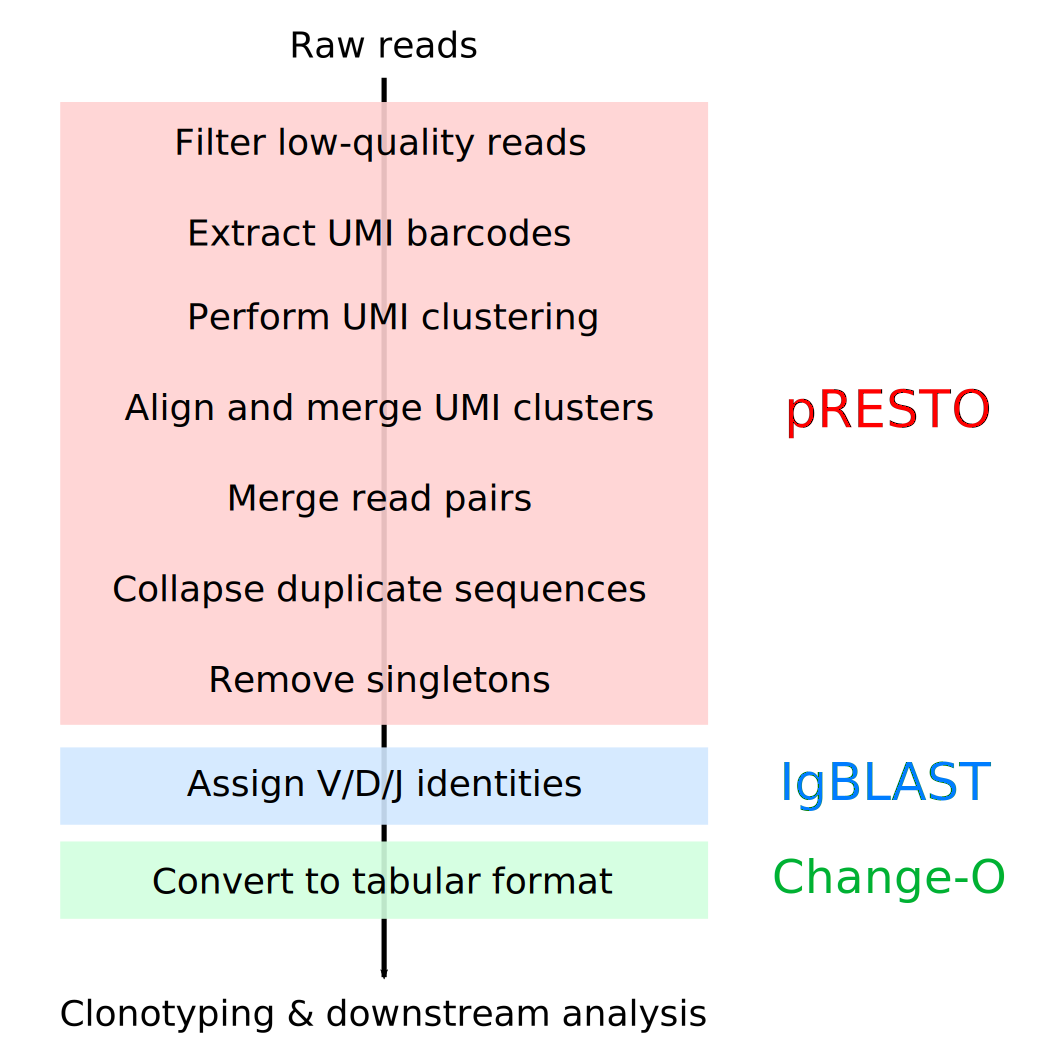
\includegraphics[width=0.6\textwidth]{_Figures/png_edited/igseq-preprocessing}
\vspace{0.5em}
\end{figure}

Raw \igseq data from the protocol described in \Cref{sec:igseq_protocol_library} takes the form of a large number of paired-end sequencing reads, each of which represents a partial, biased and error-prone sample from the set of input sequences in the original sample. To get from this fragmented and unreliable dataset to a set of complete, error-corrected and bias-adjusted \igh{} variable-region sequences, extensive pre-processing must be performed on the raw data. In this case, this pre-processing was largely carried out with \program{pRESTO} \parencite{vanderheiden2014presto}, part of the Immcantation suite of repertoire-sequencing analysis tools. % TODO: Citations for pRESTO and Immcantation

To begin with, each read pair in the dataset is annotated with various information about the source individual (ID, strain, sex, age and weight at death, etc.) as well as information about its place in the replicate structure of the experiment. The sequences are then filtered to remove low-quality sequences (with a mean Phred score of less than 20). Invariant primer sequences are trimmed from the ends of the reads, and the UMI sequence of each forward read (containing the TSA sequence) is extracted into a sequence annotation and removed from the read sequence.

As discussed in \Cref{sec:igseq_protocol_library}, the use of UMI sequences enables biases and errors in library insert sequences to be corrected by taking the consensus sequence of all reads sharing a given UMI. However, PCR and sequencing errors can also affect the sequence of the UMI itself, in which case reads that in fact belong to a single group will be spuriously separated during pre-processing; this can result in spuriously low UMI group sizes, spuriously high numbers of unique sequences, and avoidable loss of sequencing data due to reads with erroneous barcodes being discarded (as low-quality, low-read-count unique sequences) at various points in the pre-processing pipeline. In addition to these barcode \textit{errors}, barcode \textit{collisions} can occur, in which multiple distinct sequences are labelled with the same UMI sequence and spuriously grouped together during UMI grouping. This can lead to spuriously large MIGs and spuriously low numbers of unique sequences, and in extreme cases lead to the rejection and loss of entire MIGs due to an insufficiently high level of sequence identity during consensus-read generation.

In order to reduce the effect of such barcode errors and collisions on the pre-processing pipeline, primer-trimmed forward reads in this pipeline undergo clustering following extraction of UMI sequences. Firstly, reads are clustered by UMI sequence, and those with sufficiently similar UMIs are grouped together into a single cluster even if their UMIs differ slightly. Following this, read insert sequences within a given cluster are themselves clustered, and those with sufficiently different insert sequences are split apart into separate clusters. Following these clustering steps, each cluster consists of reads with highly similar barcode sequences as well as similar insert sequences; it is these clusters, rather than the raw UMI sequences, on which consensus-read generation is performed.

Following cluster inference as described above, annotations (including barcode and cluster annotations) are copied from each TSA-bearing forward-read to its mate among the reverse reads. The forward and reverse reads were then separately grouped by cluster identity and collapsed into a consensus sequence, with the contribution of each position in each read to the consensus weighted according to its quality score. % TODO: Is this actually how it works?
As most PCR and sequencing errors should be present in only a minority of the sequences descended from a given input sequence, this process effectively corrects these errors, while also removing the effect of biased amplification on observed sequence abundance. The more sequences present in a given cluster, the more effective is consensus-read generation at correcting these errors; as such, there is a trade-off inherent in the amount of oversequencing of the molecules in each library, with more oversequencing improving error correction but reducing the amount of data available. % TODO: Mention early/hotspot errors as counterexample?

Following consensus-read generation, pairs of forward and reverse consensus reads with matching cluster annotations are assembled into a single contiguous sequence, ideally covering the entire variable-region sequence of the template molecule; forward or reverse consensus reads lacking a mate in the other read set are discarded. At this point in the pipeline, each entry is assumed to represent a distinct RNA template molecule in the original sample. Sequences with different cluster annotations but matching insert sequences are then collapsed together into a single sequence, which is annotated with the number of contributing consensus reads; each sequence entry now represents a unique sequence in the dataset. Finally, unique sequences represented by only a single read pair (which could not be corrected by consensus-read generation and are therefore highly unreliable) are discarded.

At the end of the \program{pRESTO} pre-processing pipeline, the raw data has been processed into a set of complete variable-region sequences, each of which is annotated with the number of contributing reads and the number of distinct instances of that sequence found in the dataset. These sequences are then assigned V/D/J-identities through alignment to reference databases with \program{IgBLAST}. Finally, the sequences and their metadata, including annotations and V/D/J-identities, are converted by \program{Change-O} (another program from the Immcantation suite) into tabular format for efficient downstream processing and analysis (\Cref{fig:igrace-preprocessing}).

\section{Establishing \igseq in turquoise killifish: pilot study}
\label{sec:igseq_pilot}

\newcommand{\embed}[1]{\input{#1}\unskip}

In order to validate the library-preparation protocol and processing pipeline described in \Cref{sec:igseq_protocol}, as well as assess the state of the turquoise-killifish antibody repertoire in mature adults, a group of four adult male killifish from the second sample group described in \Cref{sec:igseq_samples} (specifically, fish 2-03, 2-04, 2-05 and 2-06) were selected for a pilot study. In this experiment, total RNA was isolated twice independently from each fish, and independent library preps were performed once on the first RNA isolate and twice on the second, for a total of three replicates per individual (\Cref{fig:igseq-pilot-design}). These twelve replicates were sequenced together in a single MiSeq run, yielding a total of \embed{_Figures/txt/pilot-reads-raw-total.txt} million read pairs (\embed{_Figures/txt/pilot-reads-raw-replicate-min.txt} to \embed{_Figures/txt/pilot-reads-raw-replicate-max.txt} million pairs per replicate, \embed{_Figures/txt/pilot-reads-raw-individual-min.txt} to \embed{_Figures/txt/pilot-reads-raw-individual-max.txt} million pairs per individual).

\begin{figure}
\centering
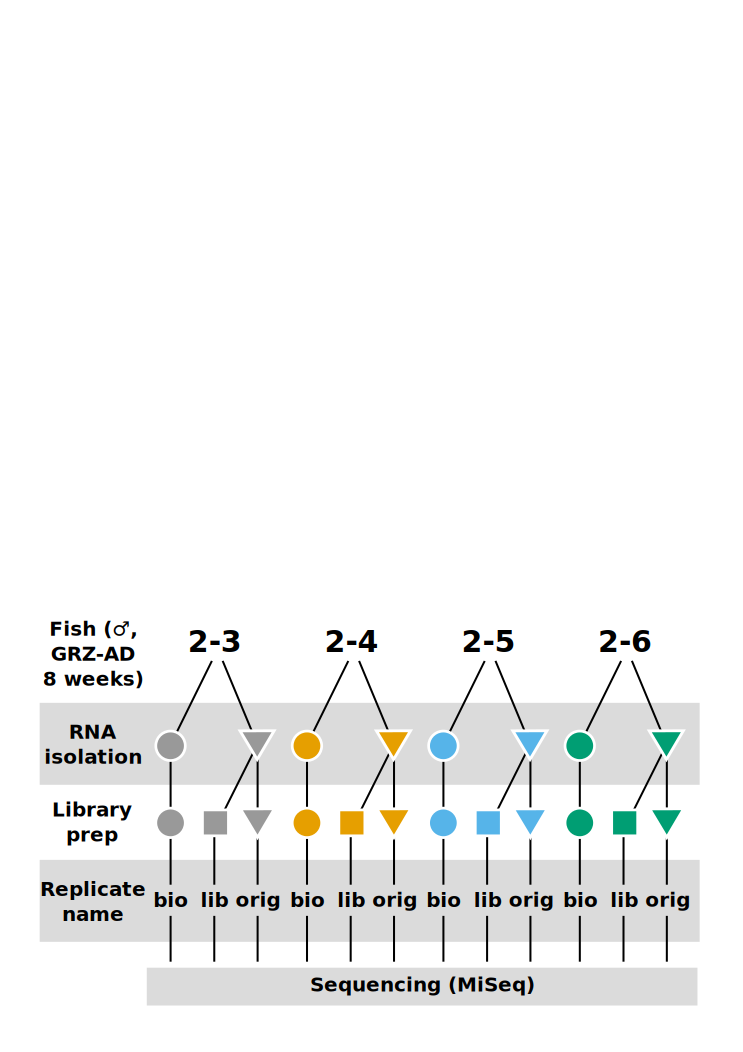
\includegraphics[width = 0.9\textwidth]{_Figures/png_edited/igseq-pilot-design_wide.png}
\caption{Experimental design of pilot study, showing relationship between replicates for each individual. Colour denotes individual of origin, while shape denotes replicate type.}
\label{fig:igseq-pilot-design}
\end{figure}

\subsection{Read survival and composition}
\label{sec:igseq_pilot_composition}

\Cref{fig:igseq-pilot-read-survival-init} shows the absolute and relative read survival for each of the twelve replicates throughout the pre-processing pipeline, up to and including VDJ assignment and Change-O table construction. The twelve replicates show relatively consistent behaviour, with \embed{_Figures/txt/pilot-read-survival-init-min.txt}\,\% to \embed{_Figures/txt/pilot-read-survival-init-max.txt}\,\% of reads surviving the entire process. Of those that do not, the biggest losses typically occur during quality filtering and removal of singleton sequences, with most other steps giving rise to relatively little sequence loss (\Cref{fig:igseq-pilot-read-survival-init-b}).

\begin{figure}
\centering
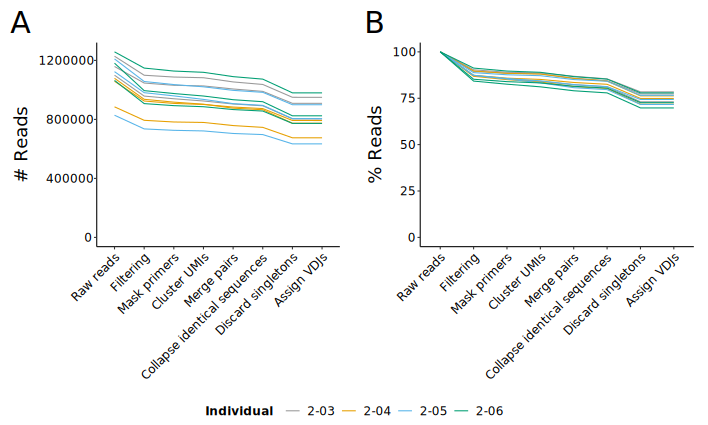
\includegraphics[width = 0.9\textwidth]{_Figures/png/pilot-read-survival-init.png}
\begin{subfigure}{0em}
\phantomsubcaption{}
\label{fig:igseq-pilot-read-survival-init-a}
\end{subfigure}
\begin{subfigure}{0em}
\phantomsubcaption{}
\label{fig:igseq-pilot-read-survival-init-b}
\end{subfigure}
\caption{Absolute (A) and relative (B) read survival during pre-processing of the pilot \igseq dataset, up to VDJ assignment and Change-O table construction.}
\label{fig:igseq-pilot-read-survival-init}
\end{figure}

In total, the pre-processed sequence repertoires of the pilot replicates contain between \embed{_Figures/txt/pilot-nseq-init-replicate-min.txt} and \embed{_Figures/txt/pilot-nseq-init-replicate-max.txt} unique sequences per replicate, corresponding to between \embed{_Figures/txt/pilot-nseq-init-individual-min.txt} and \embed{_Figures/txt/pilot-nseq-init-individual-max.txt} unique sequences per individual killifish and \embed{_Figures/txt/pilot-nseq-init-total.txt} unique sequences in total. Of these, \embed{_Figures/txt/pilot-nseq-init-pc-functional.txt}\,\% of sequences (corresponding to \embed{_Figures/txt/pilot-nreads-init-pc-functional.txt}\,\% of sequencing reads) are annotated by \program{Change-O} as functional, meaning they have successfully been assigned V- and J-identities, their V- and J-sequences are in-frame, and they do not contain any STOP codons (\Cref{fig:igseq-pilot-functional-prop-a}). A further \embed{_Figures/txt/pilot-nseq-init-pc-noj.txt}\,\% of sequences (corresponding to \embed{_Figures/txt/pilot-nreads-init-pc-noj.txt}\,\% of reads) failed to be assigned even an uncertain J-identity, meaning that no \jh sequence in the reference database aligned to the insert sequence; the remaining \embed{_Figures/txt/pilot-nseq-init-pc-other.txt}\,\% of sequences (corresponding to \embed{_Figures/txt/pilot-nreads-init-pc-other.txt}\,\% of reads) have a J-assignment but are rendered nonfunctional by an internal STOP codon and/or a frameshift between their V- and J-sequences (\Cref{fig:igseq-pilot-functional-prop-a}).

\begin{figure}
\centering
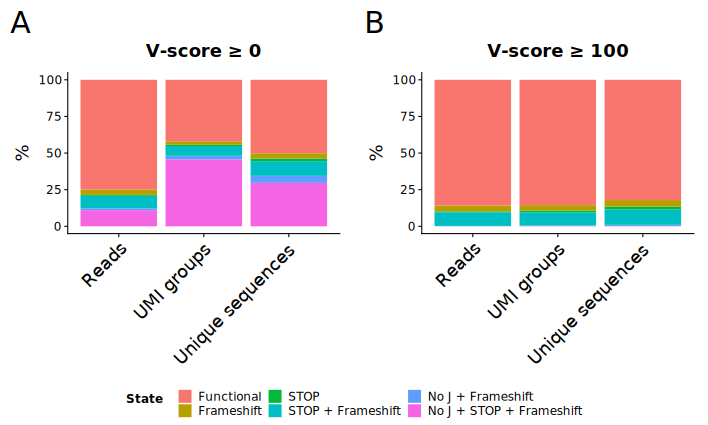
\includegraphics[width = 0.9\textwidth]{_Figures/png/pilot-functional-prop}
\begin{subfigure}{0em}
\phantomsubcaption{}
\label{fig:igseq-pilot-functional-prop-a}
\end{subfigure}
\begin{subfigure}{0em}
\phantomsubcaption{}
\label{fig:igseq-pilot-functional-prop-b}
\end{subfigure}
\caption{Proportion of input reads, UMI groups and unique sequences in the pilot \igseq dataset belonging to different (non)functional categories, before (A) and after (B) filtering on V-alignment score.}
\label{fig:igseq-pilot-functional-prop}
\end{figure}

\begin{figure}
\centering
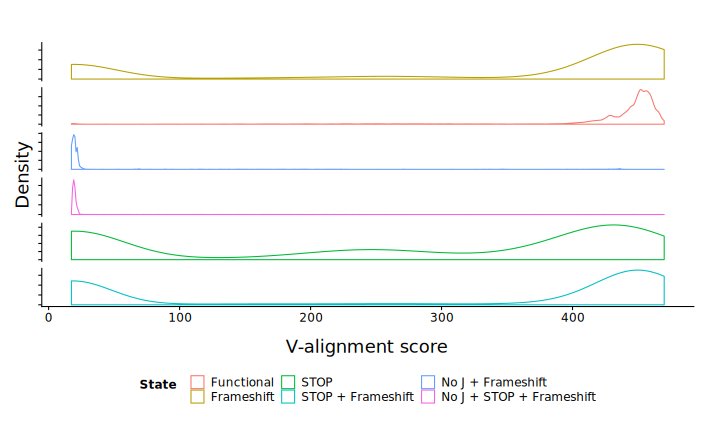
\includegraphics[width = 0.9\textwidth]{_Figures/png/pilot-functional-vscores}
\caption{Kernel density plots of distributions of V-alignment scores among unique sequences in the pilot \igseq dataset. Vertical axes are not to scale between sequence categories.}
\label{fig:igseq-pilot-functional-vscores}
\end{figure}

As genuinely recombined but nonfunctional sequences would be expected to have undergone V(D)J recombination and so have a complete J-sequence, the lack of assigned J-identities for a significant minority of sequences suggests that this subset of sequences may be artifactual, erroneous or otherwise malformed. Supporting this assumption, sequences without J-assignments overwhelmingly have very low V-alignment scores reported by \program{IgBLAST}, with an average score of \embed{_Figures/txt/pilot-vscore-mean-noj.txt} $\pm$ \embed{_Figures/txt/pilot-vscore-sd-noj.txt} (mean $\pm$ standard deviation), compared to \embed{_Figures/txt/pilot-vscore-mean-other.txt} $\pm$ \embed{_Figures/txt/pilot-vscore-sd-other.txt} for other nonfunctional sequences and \embed{_Figures/txt/pilot-vscore-mean-functional.txt} $\pm$ \embed{_Figures/txt/pilot-vscore-sd-functional.txt} for functional sequences (\Cref{fig:igseq-pilot-functional-vscores}). A simple V-score cut-off of 100, therefore, effectively removes the vast majority of these low-quality sequences, while leaving the population of functional sequences intact (\Cref{fig:igseq-pilot-functional-prop-b}); in total, \embed{_Figures/txt/pilot-nseq-init-dropped-vscore.txt} unique sequences, corresponding to \embed{_Figures/txt/pilot-read-survival-rel-loss-total.txt}\,\% of input reads, were removed in this way.

\begin{figure}
\centering
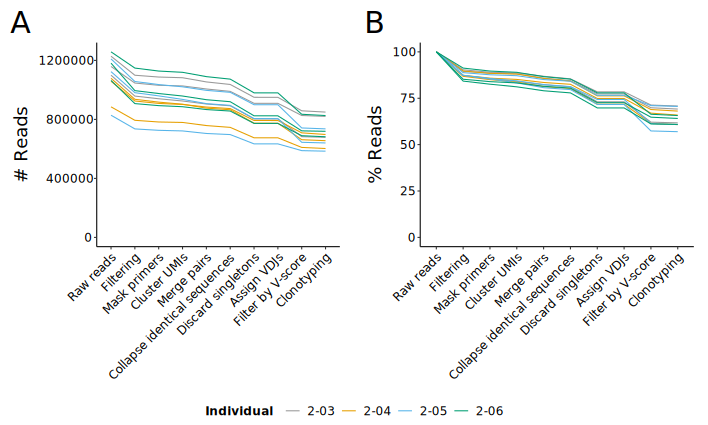
\includegraphics[width = 0.9\textwidth]{_Figures/png/pilot-read-survival-all.png}
\begin{subfigure}{0em}
\phantomsubcaption{}
\label{fig:igseq-pilot-read-survival-all-a}
\end{subfigure}
\begin{subfigure}{0em}
\phantomsubcaption{}
\label{fig:igseq-pilot-read-survival-all-b}
\end{subfigure}
\caption{Absolute (A) and relative (B) read survival during pre-processing of the pilot \igseq dataset, up to and including ....} % TODO: Decide on last step: clonotyping or functionality?
\label{fig:igseq-pilot-read-survival-all}
\end{figure} % TODO: Reference this figure in text

\subsection{Clonotyping} % TODO: Better section title
\label{sec:igseq_pilot_clones}

Following assignment of VDJ identities and quality filtering, sequences in an antibody repertoire can be assigned to clones: groups of B-cells descended from a single \naive B-cell ancestor, and therefore sharing a single VDJ-recombination event. Sequences in the same clone are said to share a \textit{clonotype}. In \program{Change-O}, clonotyping is performed by dividing sequences into groups sharing a consistent V-assignment, J-assignment and CDR3 length, then each group undergoes single-linkage clustering based on Hamming distance between CDR3 sequences. To identify a distance threshold for cutting the cluster dendrogram, ... % TODO: describe thresholding algorithm.
% In addition to giving information about the common ancestry of groups of B-cells, clonotyping also allows V/D/J-calls of repertoire sequences to be improved by ...

One disadvantage of single-linkage clustering in this context is that non-informative \sequence{N} positions can result in artifactual links between unrelated sequences. As such, sequences with a large number of junctional \sequence{N} positions can significantly disrupt the clonotyping process. On the other hand, as over \embed{_Figures/txt/pilot-filtered-nn-any.txt}\,\% of unique sequences in the pilot dataset contain at least one such junctional \sequence{N} position, excluding them all would represent a significant loss of data. In order to minimise the number of discarded sequences while also minimising the disrupting effects of sequences with junctional \sequence{N}s, sequences with exactly one junctional \sequence{N} position (comprising \embed{_Figures/txt/pilot-filtered-1n-total.txt}\,\% of total sequences and \embed{_Figures/txt/pilot-filtered-1n-withn.txt}\,\% of sequences with at least one junctional \sequence{N}; \Cref{tab:igseq-pilot-filtered-nn}) were included in the clonotyping process for the pilot dataset, while those with two or more junctional \sequence{N} positions were excluded. This procedure successfully assigned clonal identities to \embed{_Figures/txt/pilot-nseq-assigned-clones.txt}\,\% of unique sequences in the V-score-filtered dataset.

\begin{table}
\caption{Distribution of junctional \sequence{N} positions in the V-score-filtered pilot dataset.}
\label{tab:igseq-pilot-filtered-nn}
% latex table generated in R 3.5.2 by xtable 1.8-3 package
% Wed Apr  3 14:27:33 2019
\begin{tabular}{lrrr}
  \toprule \# junctional Ns & \# unique sequences & \% of all sequences & \% of sequences with $>$0 junctional Ns \\ 
  \midrule 0 & 49134 & 88.924 & 0.00 \\ 
  1 & 3388 & 6.132 & 67.94 \\ 
  2 & 961 & 1.739 & 19.27 \\ 
  3 & 324 & 0.586 & 6.50 \\ 
  4 & 125 & 0.226 & 2.51 \\ 
  5 & 93 & 0.168 & 1.86 \\ 
  $>$5 & 96 & 0.174 & 1.93 \\ 
   \bottomrule \end{tabular}

\end{table}

In total, \embed{_Figures/txt/pilot-nclones-individual-min.txt} to \embed{_Figures/txt/pilot-nclones-individual-max.txt} clones were identified per individual fish in the pilot dataset. As expected, the clone-size distribution is overwhelmingly dominated by small clones (\Cref{fig:igseq-pilot-clone-sizes-sizes}): across all individuals, \embed{_Figures/txt/pilot-nclones-pc-1count.txt}\,\% of clones are observed as just a single unique sequence across all replicates, while \embed{_Figures/txt/pilot-nclones-pc-small.txt}\,\% contain fewer than five unique sequences. As a result, the great majority of clones (\embed{_Figures/txt/pilot-nclones-pc-1rep.txt}\,\%) are observed in only a single replicate per individual, with \embed{_Figures/txt/pilot-nclones-pc-2rep.txt}\,\% present in two replicates and \embed{_Figures/txt/pilot-nclones-pc-3rep.txt}\,\% shared across all three. Unsurprisingly, however, larger clones are much more likely to be shared across multiple replicates (\Cref{fig:igseq-pilot-clone-sizes-reps}), consistent with a model in which a large number of small clones are sampled only rarely while a much smaller number of large clones is sampled much more often. Overall, the level of agreement between the replicates is high (\Cref{fig:igseq-pilot-clone-sizes-cor-boxplots,fig:igseq-pilot-clone-sizes-cor-scatter}), with an average inter-replicate correlation in clone size of $r=\embed{_Figures/txt/pilot-clone-sizes-cor-avg.txt}$.

\begin{figure}
\centering
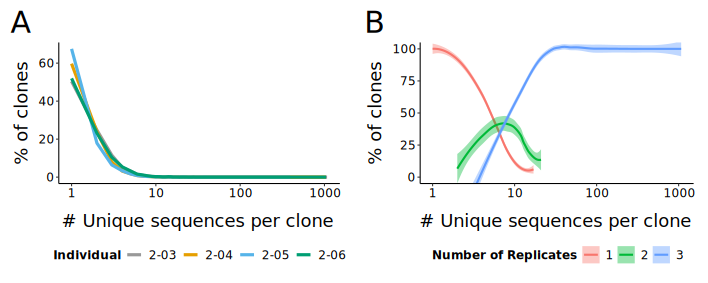
\includegraphics[width = 0.9\textwidth]{_Figures/png/pilot-clone-sizes}
\begin{subfigure}{0em}
\phantomsubcaption{}
\label{fig:igseq-pilot-clone-sizes-sizes}
\end{subfigure}
\begin{subfigure}{0em}
\phantomsubcaption{}
\label{fig:igseq-pilot-clone-sizes-reps}
\end{subfigure}
\caption{(A) Proportion of clones of different sizes for each individual in the pilot dataset, measured in unique sequences per clone. (B) Proportion of clones of each size found across one, two or all three replicates of the appropriate individual.}
% TODO: Add suitable overall figure title
\label{fig:igseq-pilot-clone-sizes}
\end{figure}

\begin{figure}
\centering
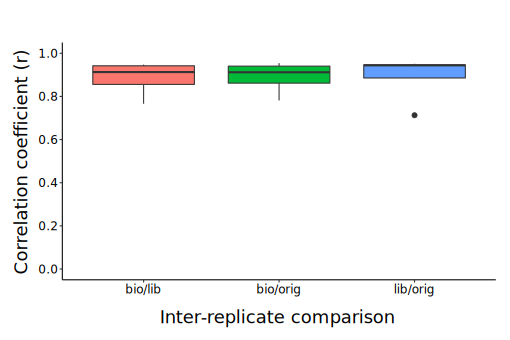
\includegraphics[width = 0.7\textwidth]{_Figures/png/pilot-clone-sizes-cor-boxplots}
\caption{Boxplots showing distribution of Pearson's product-moment correlation coefficients of clone sizes for each pair of replicates, as measured by the number of unique sequences per clone in each replicate. Clones absent in a given replicate were given a size of zero.}
% TODO: Add suitable overall figure title
\label{fig:igseq-pilot-clone-sizes-cor-boxplots}
\end{figure}

\begin{figure}
\centering
\includegraphics[width = 0.7\textwidth]{_Figures/png/pilot-clone-sizes-cor-scatter}
\caption{Scatter plots comparing clone sizes across biological replicates for each individual in the pilot dataset.}
% TODO: Add suitable overall figure title
\label{fig:igseq-pilot-clone-sizes-cor-scatter}
\end{figure}

One of the most startlingly reproducible findings of immune-repertoire-sequencing studies across multiple species has been the rank:frequency distribution of clonotypes, which consistently follows a Zipf distribution; that is, the frequency of the $k$th largest clone in a repertoire dataset containing $N$ total clones is well-predicted by:

\begin{equation}
f(k | N, s) = \frac{x^{-s}}{H_{N,s}}
\end{equation}

\noindent for some exponent parameter $s > 0$, where $H_{N,s}$ is the $N$th generalised harmonic number of order $s$. This power-law distribution of clone sizes is inconsistent with clonal expansion under neutral selection and instead suggests that clone sizes evolve within a complex and fluctuating fitness landscape. % TODO: Read Desponds source for this

In turquoise killifish repertoires, the vast majority of clones correspond well to a Zipf distribution of clone sizes, consistent with observations from other vertebrate species (\Cref{{fig:igseq-pilot-clones-zipf}}). % TODO: Fit figure for this
However, the largest two to six clones from each individual are consistently much larger than predicted by the best-fit Zipf distribution for the rest of the dataset, suggesting \dots. % TODO: What exactly is this suggesting.

\begin{figure}
\centering
\includegraphics[width=0.9\textwidth]{_Figures/png/pilot-clones-zipf}
\caption{Log-log plots of clonal rank versus relative frequency in the repertoire of each individual in the pilot dataset, with both rank and frequency measured in terms of number of unique sequences per clone. The black lines give the expected rank-frequency distribution under the maximim-likelihood estimate Zipf distribution for each individual, with expanded clones obviously deviating from such a distribution (indicated by crosses) excluded from the estimation procedure.}
\label{fig:igseq-pilot-clones-zipf}
\end{figure} % TODO: Describe MLE procedure

... recommend ... % D20, overabundance plots, public clones

\Cref{fig:igseq-pilot-clone-diversity} shows the diversity of clone sizes in each individual in the pilot dataset, as measured using Hill diversity spectra (\Cref{?}). % TODO: Refer to diversity appendix here
\Cref{fig:igseq-pilot-clone-diversity-alpha} gives the alpha diversity, or average diversity \textit{across} replicates for each individual, while \Cref{fig:igseq-pilot-clone-diversity-beta} shows the beta-diversity, or variation in clone-size distribution \textit{between} replicates. In both cases, each curve represents a single individual and gives the corresponding diversity measure at a range of different diversity orders; roughly speaking, higher diversity orders place proportionately more weight on common over rare species (i.e. clones) when calculating diversity, with zero-order diversity being equivalent to simple species richness. As beta-diversity (unlike alpha-diversity) is sensitive to the number of sub-populations being compared, it has been rescaled here such that 0 represents the minimum possible diversity measure and 1 represents the maximum (\Cref{?}). % TODO: Explain rescaling in diversity appendix

... % TODO: Interpret alpha-diversity curve, after deciding how to interpret more meaningful curves from other experiments; give Shannon-entropy scores

Unlike alpha-diversity, the beta-diversity spectrum of a population does not necessarily decline monotonically with increasing diversity order; nevertheless, in \Cref{fig:igseq-pilot-clone-diversity-beta} the between-replicate beta-diversity is much higher at low diversity orders (where it approaches the maximum) than at higher ones (where it is close to the minimum). This indicates that replicates from the same individual are show very different clonal distributions when all clones are included, but that these ditributions become increasingly similar as more and more weight is put on the largest clones in each replicate. This result is highly consistent with the findings in \Cref{fig:igseq-pilot-clone-sizes} that each repertoire contains a small number of large clones (which are shared reproducibly between replicates) and a much larger number of much smaller clones (which are not); the difference in patterns of cross-replicate reproducibility between small and large clones observed in \Cref{fig:igseq-pilot-clone-sizes-reps} gives rise to the patterns of beta-diversity observed in \Cref{fig:igseq-pilot-clone-diversity-beta}.

\begin{figure}
\centering
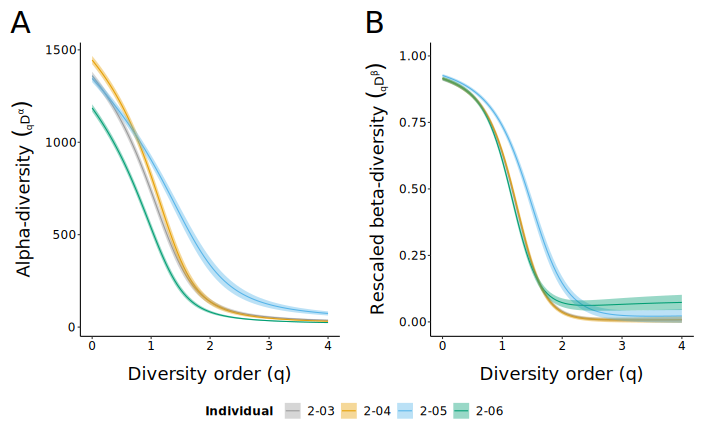
\includegraphics[width = 0.9\textwidth]{_Figures/png/pilot-clone-diversity}
\begin{subfigure}{0em}
\phantomsubcaption{}
\label{fig:igseq-pilot-clone-diversity-alpha}
\end{subfigure}
\begin{subfigure}{0em}
\phantomsubcaption{}
\label{fig:igseq-pilot-clone-diversity-beta}
\end{subfigure}
\caption{\textbf{Clonal diversity spectra for pilot dataset:} Hill diversity spectra of clone sizes (as measured by number of unique sequences per clone) over replicates for each individual in the pilot dataset. (A) Alpha-diversity across replicates; (B) Beta-diversity across replicates, rescaled to between 0 (minimum) and 1 (maximum) for each individual.}
\label{fig:igseq-pilot-clone-diversity}
\end{figure}

\subsection{V(D)J segment usage}

The clonal repertoire of an organism reflects the history of \naive B-cell production and subsequent clonal expansion in that individual, and as such is unique to each individual repertoire: by definition, clones cannot be shared between individuals. As such, while an important tool for ...
(and a useful way to assess reproducibility between replicates),
clonal measures are limited in their ability to meaningfully compare the antibody repertoires of different individuals. 

In contrast, the range of V(D)J-combinations available within an antibody repertoire is defined by the corresponding gene locus (\Cref{?}) % TODO: See locus chapter
and is therefore largely shared across individuals of a given species. This is particularly true for inbred lines of laboratory model organisms, for which the high level of polymorphism observed in the V-regions of wild populations % TODO: Cite this
is not an issue. As such, the V(D)J usage distributions of antibody repertoires represent an alternative metric for measuring repertoire composition and diversity, which is more amenable to comparison between individuals (and groups of individuals) of the same species.

The Repertoire Dissimilarity Index (RDI) % TODO: Cite this
is a method for computing a distance between any two repertoires on the basis of their V(D)J segment composition, based on the Euclidean distance between their respective V(D)J-abundance vectors. As such, it provides a pairwise distance metric which can be used to compare, cluster and visualise the relationship between different antibody repertoires. Two methods for visualising the RDI distances between pilot replicates are shown in \Cref{fig:igseq-pilot-rdi}: in \Cref{fig:igseq-pilot-rdi-dendro}, the replicates are arranged in a dendrogram by average-linkage clustering over their pairwise RDI distances, while for \Cref{fig:igseq-pilot-rdi-pcoa} the same distances were used to compute a principal co-ordinate analysis, % TODO: Cite this
of which the first two co-ordinates are visualised here. In both cases, replicates from the same individual clearly cluster together compared to replicates from different individuals, demonstrating the inter-replicate reproducibility of the \igseq protocol.

\begin{figure}
\centering
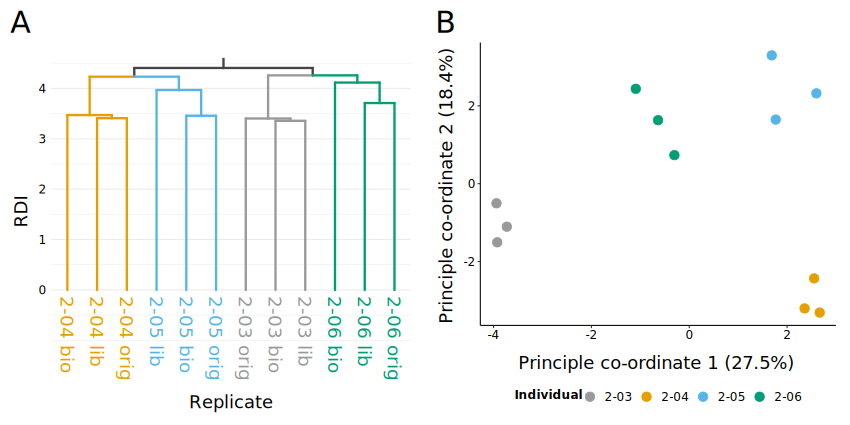
\includegraphics[width = 0.9\textwidth]{_Figures/png/pilot-rdi-VDJ}
\begin{subfigure}{0em}
\phantomsubcaption{}
\label{fig:igseq-pilot-rdi-dendrogram}
\end{subfigure}
\begin{subfigure}{0em}
\phantomsubcaption{}
\label{fig:igseq-pilot-rdi-pcoa}
\end{subfigure}
\caption[Repertoire dissimilarity index (RDI) analysis of pilot data]{\textbf{Repertoire dissimilarity index (RDI) analysis of pilot data:} (A) Dendrogram of pilot replicates produced through average-linkage clustering on pairwise RDI distances. (B) Principal co-ordinate analysis (PCoA) of pairwise RDI distances between pilot replicates, coloured by source individual.}
\label{fig:igseq-pilot-rdi}
\end{figure}

% TODO: Depict and describe V(D)J diversity spectra;  compare beta to cross-replicate spectra

\subsection{Generative models and potential repertoire entropy}

The previous two sections analysed clonal and V(D)J repertoires, respectively, as actually observed for individuals in the pilot dataset. For several reasons, such observed distributions are distinct from the original generative process giving rise to ...


The observed V(D)J repertoire is strongly affected by selection, clonal expansion and other population-level processes taking place after the initial generation of \igh{} sequences via VDJ-recombination and its attendant junctional diversity...

In order to access the original generative process giving rise to recombined \igh{} sequences in an organism, the program \program{IGoR} (...) infers a generative model of sequence recombination ... % TODO: Describe IGoR process, sequence selection


% TODO: Replicability (RDI, beta-spectra), alpha-spectra

% TODO: Generative models

% TODO: SHM, selection

% 1. Establishing IgSeq in TK
% - Library prep protocol design
% - Principles (template switching, UMIs, adaptor attachment, size-selection)
% - Testing (e.g. TapeStation, Sanger seq)

% 2. Validating IgSeq in TK
% - Sample collection & RNA extraction
% - Study design
% - Bioinformatic pipeline summary

% 3. Baseline results (pilot)

% 4. Ageing cohort results
% - Study design
% - Diversity
% - Generative models
% - SHM
% - Clonality
% - ???

% 5. uBiome results
% - Study design
% - Diversity
% - Generative models
% - SHM etc
% - Relate to uBiota?

\section{The effect of ageing on turquoise killifish antibody repertoires}
\label{sec:igseq_ageing}

The result of the pilot experiment described in \Cref{sec:igseq_pilot} demonstrated that \Igseq sequencing of turquoise killifish... % TODO: Briefly summarise importance of pilot results

In order to investigate the effect of ageing on these processes, each of the 32 fish % TODO: Include/exclude group 4?
sacrificed in \Cref{sec:igseq_samples} underwent two independent library preparations as described in \Cref{sec:igseq_protocol_library}, % TODO: Table of cycle numbers etc.
for a total of 64 pooled libraries; these were then sequenced together in two MiSeq runs, yielding a total of \embed{_Figures/txt/ageing-reads-raw-total.txt} million read pairs (\embed{_Figures/txt/ageing-reads-raw-replicate-min.txt} to \embed{_Figures/txt/ageing-reads-raw-replicate-max.txt} million pairs per replicate, \embed{_Figures/txt/ageing-reads-raw-individual-min.txt} to \embed{_Figures/txt/ageing-reads-raw-individual-max.txt} million pairs per individual), and the resulting reads underwent pre-processing, filtering and clonotyping as described in \Cref{sec:igseq_protocol_preprocess,sec:igseq_pilot_composition,sec:igseq_pilot_clones}. 

\Cref{fig:igseq-ageing-read-survival-all} shows the absolute and relative read survival for each of the sixty-four sequencing libraries throughout this process. As with the pilot dataset, the replicates show relatively consistent behaviour up to and including VDJ assignment and Change-O database construction, with \embed{_Figures/txt/ageing-read-survival-init-min.txt}\,\% to \embed{_Figures/txt/ageing-read-survival-init-max.txt}\,\% of reads surviving up to this stage in the pipeline. However, a somewhat % TODO: much?
 larger number of sequences (\embed{_Figures/txt/ageing-read-survival-rel-loss-total.txt}\,\%, up to \embed{_Figures/txt/ageing-read-survival-rel-loss-max.txt}\,\% per replicate) are lost during V-score filtering compared to the pilot dataset (\embed{_Figures/txt/pilot-read-survival-rel-loss-total.txt}\,\%, up to \embed{_Figures/txt/pilot-read-survival-rel-loss-max.txt}\,\% per replicate). This inconsistency is due to a greater preponderance in the ageing dataset of malformed, J-identity-lacking sequences, which in this case actually make up an absolute majority of unique sequences in the \program{pRESTO}-processed dataset (\Cref{fig:igseq-ageing-functional-prop-pre}). After filtering on V-score, however, the functional composition of the ageing dataset is similar to that of the pilot data (\Cref{fig:igseq-ageing-functional-prop-post,fig:igseq-pilot-functional-prop-b}).

\begin{figure}
\centering
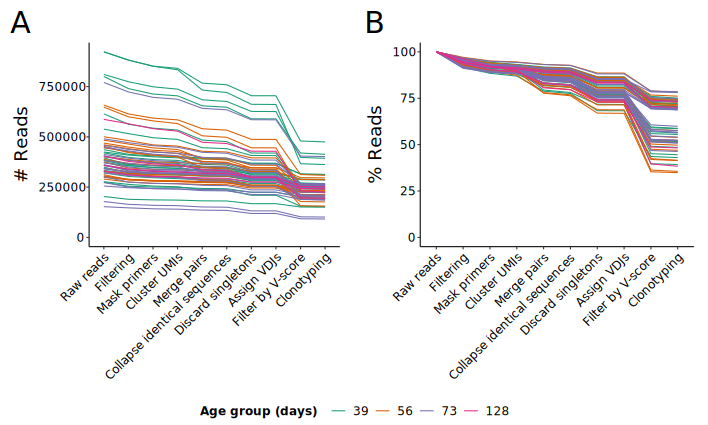
\includegraphics[width = 0.9\textwidth]{_Figures/png/ageing-read-survival-all.png}
\begin{subfigure}{0em}
\phantomsubcaption{}
\label{fig:igseq-ageing-read-survival-all-abs}
\end{subfigure}
\begin{subfigure}{0em}
\phantomsubcaption{}
\label{fig:igseq-ageing-read-survival-all-rel}
\end{subfigure}
\caption{Absolute (A) and relative (B) read survival during pre-processing of the \igseq ageing dataset, up to and including clonotyping.}
\label{fig:igseq-ageing-read-survival-all}
\end{figure} % TODO: Get age-group colour scheme

\begin{figure}
\centering
\includegraphics[width = 0.9\textwidth]{_Figures/png/ageing-functional-prop}
\begin{subfigure}{0em}
\phantomsubcaption{}
\label{fig:igseq-ageing-functional-prop-pre}
\end{subfigure}
\begin{subfigure}{0em}
\phantomsubcaption{}
\label{fig:igseq-ageing-functional-prop-post}
\end{subfigure}
\caption{Proportion of input reads, UMI groups and unique sequences in the \igseq ageing dataset belonging to different (non)functional categories, before (A) and after (B) filtering on V-alignment score.}
\label{fig:igseq-ageing-functional-prop}
\end{figure}

Following V-score filtering, \embed{_Figures/txt/ageing-nseq-assigned-clones.txt}\,\% of unique sequences in the ageing dataset were successfully assigned clonal identities. The number of clones inferred per individual ranged from \embed{_Figures/txt/ageing-nclones-individual-min.txt} to \embed{_Figures/txt/ageing-nclones-individual-max.txt}, with a median of \embed{_Figures/txt/ageing-nclones-individual-med.txt}. This is somewhat lower than the median of \embed{_Figures/txt/pilot-nclones-individual-med.txt} clones per individual for the pilot study, reflecting the lower number of reads per individual available in this dataset; for comparison, for the four individuals included in the pilot study, the number of identified clones in the ageing dataset ranges from \embed{_Figures/txt/ageing-nclones-individual-min-pilot.txt} to \embed{_Figures/txt/ageing-nclones-individual-max-pilot.txt}.
% TODO: Boxplot of clone counts across age groups
Concordantly, the distribution of clone sizes detected is even more skewed towards small clones than in the pilot dataset: \embed{_Figures/txt/ageing-nclones-pc-1count.txt}\,\% of clones are observed as just a single unique sequence across all replicates, while \embed{_Figures/txt/ageing-nclones-pc-small.txt}\,\% contain fewer than five unique sequences (\Cref{fig:igseq-ageing-clone-sizes-sizes}). As in the pilot dataset, larger clones were much more likely to be observed across both replicates for a given individual  (\Cref{fig:igseq-ageing-clone-sizes-reps}).

% TODO: Discuss inter-replicate correlational pattern
% TODO: Discuss Zipf fit

\begin{figure}
\centering
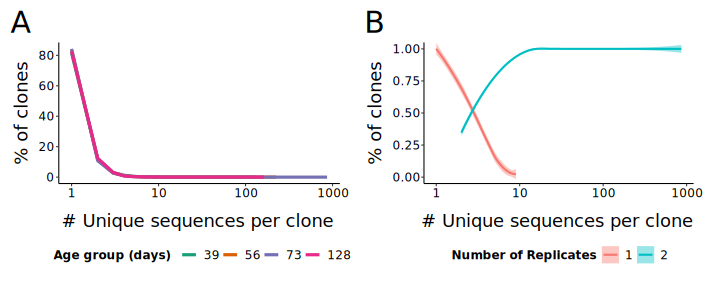
\includegraphics[width = 0.9\textwidth]{_Figures/png/ageing-clone-sizes}
\begin{subfigure}{0em}
\phantomsubcaption{}
\label{fig:igseq-ageing-clone-sizes-sizes}
\end{subfigure}
\begin{subfigure}{0em}
\phantomsubcaption{}
\label{fig:igseq-ageing-clone-sizes-reps}
\end{subfigure}
\caption{(A) Proportion of clones of different sizes for each individual in the ageing dataset, measured in unique sequences per clone. (B) Proportion of clones of each size found across one or both replicates of the appropriate individual.}
% TODO: Add suitable overall figure title
\label{fig:igseq-ageing-clone-sizes}
\end{figure}

In order to assess the effect of age on the clonal diversity of killifish antibody repertoires, the alpha-diversity spectrum of each age group was computed as described in ... . The result, shown in \Cref{fig:igseq-ageing-clone-diversity-alpha}, suggests that repertoire diversity declines monotonically between 5.5 and 10.5 weeks of age in the turquoise killifish, with the most rapid decline observed between 8 and 105 weeks: across the entire spectrum, the alpha-diversity of the 8-week group is the same as or lower than that of the 5.5 week group, the 10.5-week group is markedly less diverse than the 8-week group, and the 18-week and 10.5-week groups exhibit similar diversity. These observations suggest a model in which repertoire diversity begins declining before or at reproductive maturation (c. 5 weeks post-hatching), declines rapidly in later adulthood, and reaches a plateau of low diversity late in life; however, the smaller size of the 18-week-old group in comparison to the others means that the patterns observed in this group cannot be taken with confidence, and it is possible that a further decline after 10.5 weeks would be observed in a larger sample.

Hill diversity spectra like the one shown in \Cref{fig:igseq-ageing-clone-diversity-alpha} are useful in that they allow the diversity across a wide range of diversity indices to be compared simultaneously. However, when comparing alpha-diversities across sample groups, by-eye comparisons of apparent diversities is of course not sufficient for concluding that a significant difference in diversity exists. Ideally, the entire shape of the diversity spectrum would be compared between groups to test for a significant difference in distribution; however, the unusual and non-parametric nature of the Hill spectrum makes such a holistic comparison difficult, and established tests for such a difference do not, to this author's knowledge, yet exist. However, it is possible to use established statistical methods to test for a difference in Hill diversity at one or more specific diversity orders, and so to obtain a partial overview of significant differences for particular aspects of each group's diversity profile.

In this case, the distributions of Hill diversity measurements at each of six diversity orders (0, 1, 1.5, 2, 3 and 4) were compared across age groups via two distinct methods. In the first, a generalised linear model of diversity \textit{versus} age-at-death was fitted to each diversity order under a gamma distribution, and the resulting model was compared to a null (intercept-only) model to test for a significant ageing term (\Cref{fig:igseq-ageing-clone-diversity-solo-fit-gamma}); in the second, a non-parametric Kruskal-Wallis analysis of variance was used, again to test for a significant effect of age-at-death on the distribution of Hill diversities at a given diversity order. Both results gave roughly consistent results, as did GLM-based methods assuming a linear or inverse-Gaussian distribution (\Cref{fig:igseq-ageing-clone-diversity-solo-fit-linear,fig:igseq-ageing-clone-diversity-solo-fit-igauss}): in all cases, a significant effect of age on diversity is found for all tested diversity orders above 1, but not for order 0 (species richness) or order 1 (exponential Shannon entropy). This pattern, which suggests a significant age effect at higher but not lower diversity orders, suggests that such an effect is driven more by expansion of large clones (which primarily affects higher-order diversity measures) than a decrease in the number of smaller clones (which primarily affects lower-order measures like species richness); if this is the case, it would accord with earlier findings of persistent clonal expansions of activated cells in aged B-cell repertoires in other model systems. % TODO: Citation needed

\begin{figure}
\centering
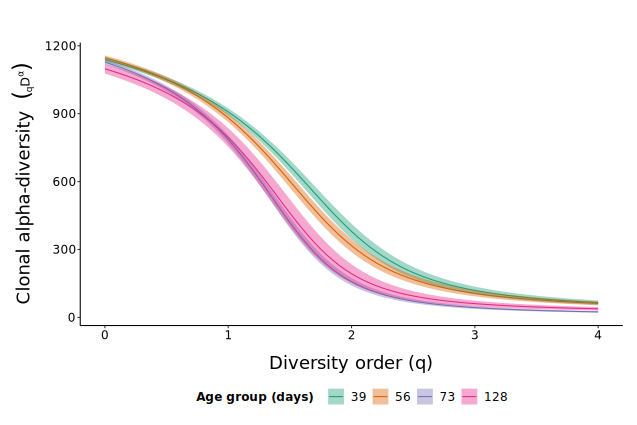
\includegraphics[width = 0.9\textwidth]{_Figures/png/ageing-clone-diversity-alpha}
\caption{\textbf{Killifish alpha-diversity declines with age:} Bootstrapped alpha-diversity spectra of clone sizes for each age group in the \igseq ageing dataset, as measured by number of unique sequences per clone.}
\label{fig:igseq-ageing-clone-diversity-alpha}
\end{figure}

\begin{figure}
\centering
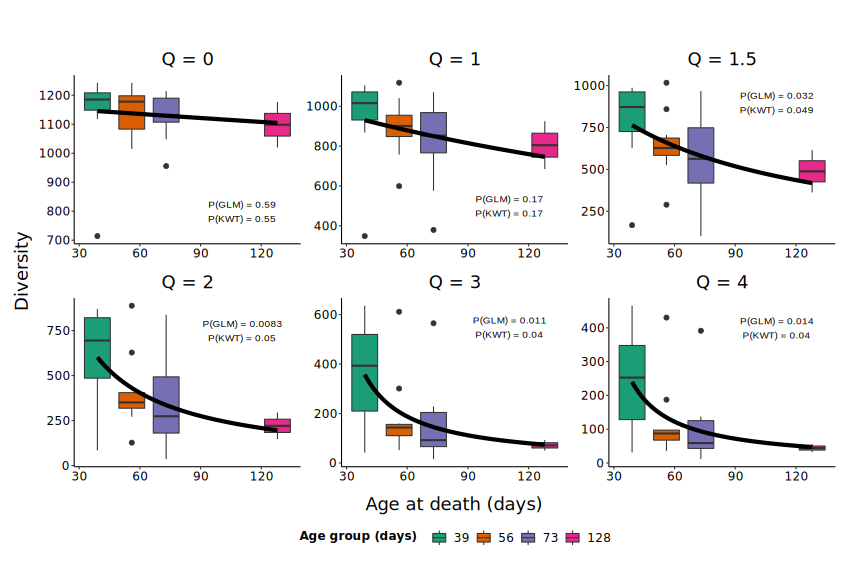
\includegraphics[width = 0.9\textwidth]{_Figures/png/ageing-clone-diversity-solo-fit-gamma}
\caption{Boxplots of Hill diversity values for the antibody repertoires of individuals of each age group in the \igseq ageing dataset at a sample of diversity orders, overlaid with the predictions of the best-fit Gamma-distributed generalised linear model at each order.  Annotated $p$-values indicate the statistical significance of the estimated age effect on diversity under the GLM ($P(GLM)$) and a Kruskal-Wallis test ($P(KWT)$) for each diversity order.}
\label{fig:igseq-ageing-clone-diversity-solo-fit-gamma}
\end{figure}

\begin{figure}
\centering
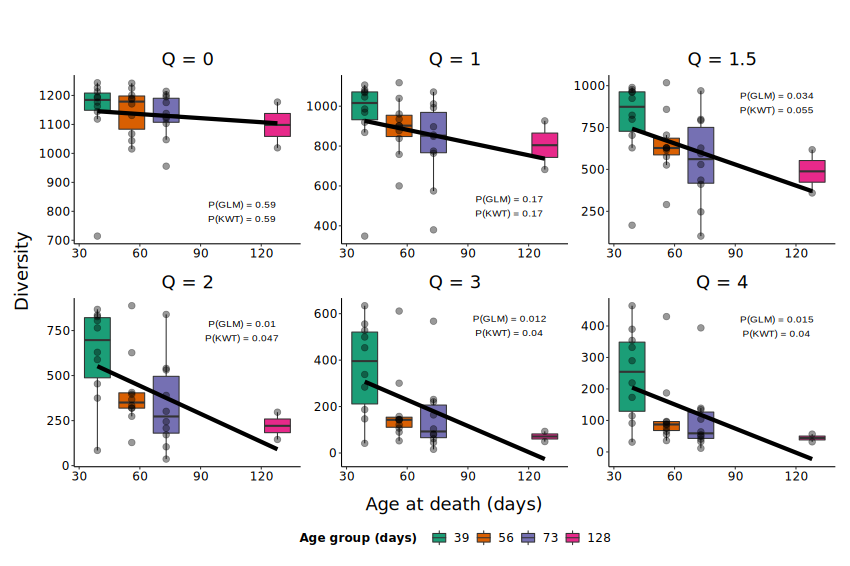
\includegraphics[width = 0.9\textwidth]{_Figures/png/ageing-clone-diversity-solo-fit-linear}
\caption{Boxplots of Hill diversity values for the antibody repertoires of individuals of each age group in the \igseq ageing dataset at a sample of diversity orders, overlaid with the predictions of the best-fit linear model at each order.}
\label{fig:igseq-ageing-clone-diversity-solo-fit-linear}
\end{figure}

\begin{figure}
\centering
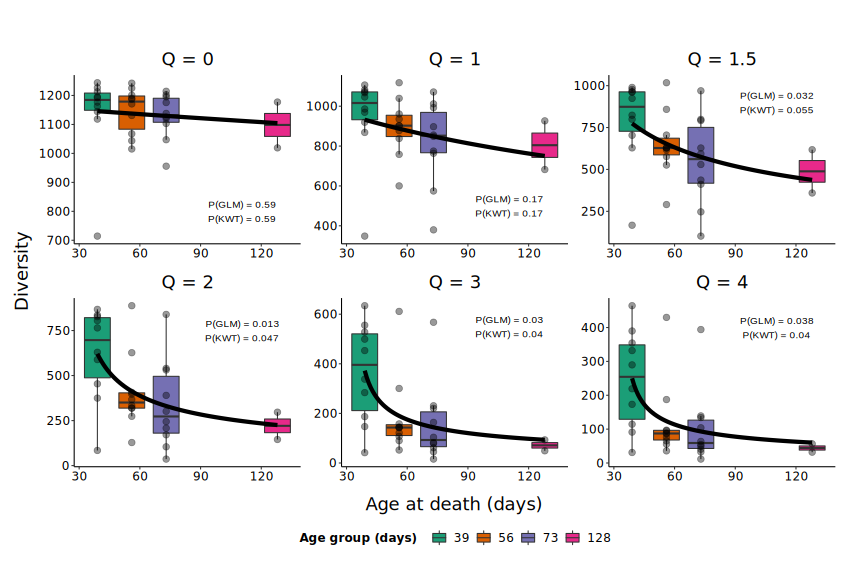
\includegraphics[width = 0.9\textwidth]{_Figures/png/ageing-clone-diversity-solo-fit-igauss}
\caption{Boxplots of Hill diversity values for the antibody repertoires of individuals of each age group in the \igseq ageing dataset at a sample of diversity orders, overlaid with the predictions of the best-fit inverse-Gaussian-distributed GLM at each order.}
\label{fig:igseq-ageing-clone-diversity-solo-fit-igauss}
\end{figure}

While a significant decline in clonal diversity was age was found at various diversity orders, no such decline was observed in the VJ-repertoires of the different age-groups, either when visually comparing the alpha-spectra (\Cref{fig:igseq-ageing-VJ-diversity-alpha}) or statistically comparing the distributions at different diversity orders (\Cref{fig:igseq-ageing-VJ-diversity-solo-fit-gamma}). This marked difference between the clonal and VJ repertoires is surprising, as a distortion in the clonal repertoire caused by an increased dominance of a few large clones would be expected to cause a similar distortion in the VJ repertoire; however, it may be the case that ... . % TODO: Explanation for this

\begin{figure}
\centering
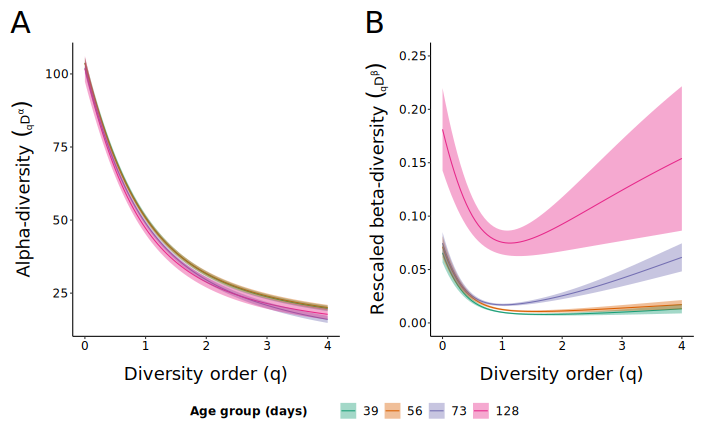
\includegraphics[width = 0.9\textwidth]{_Figures/png/ageing-VJ-diversity-alpha-beta}
\begin{subfigure}{0em}
\phantomsubcaption{}
\label{fig:igseq-ageing-VJ-diversity-alpha}
\end{subfigure}
\begin{subfigure}{0em}
\phantomsubcaption{}
\label{fig:igseq-ageing-VJ-diversity-beta}
\end{subfigure}
\caption{\textbf{VJ-diversity spectra for ageing dataset:} Hill diversity spectra of VJ usage (as measured by number of unique sequences per unambiguous VJ identity) over individuals for each age group in the \igseq ageing dataset. (A) Alpha-diversity across individuals; (B) Beta-diversity across individuals, rescaled to between 0 (minimum) and 1 (maximum) in accordance with the number of individuals in each age group.}
\label{fig:igseq-ageing-VJ-diversity-spectra}
\end{figure}

\begin{figure}
\centering
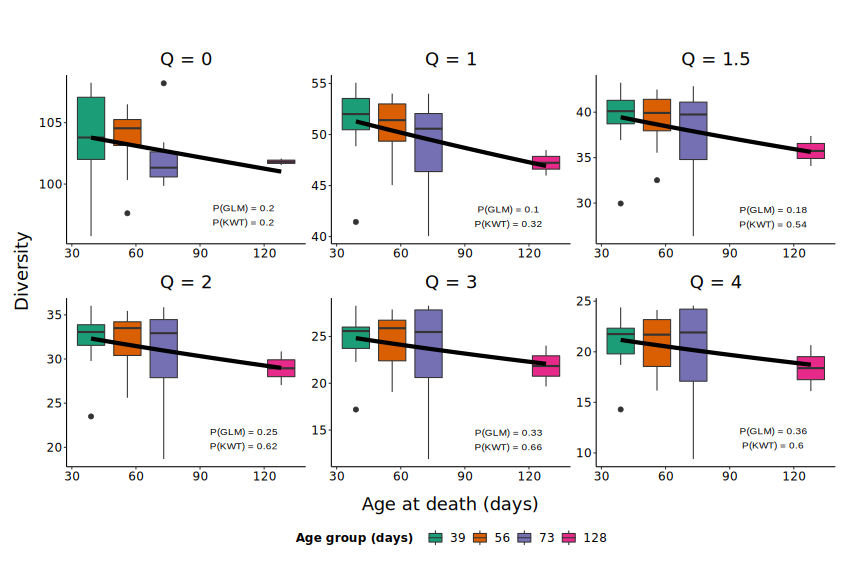
\includegraphics[width = 0.9\textwidth]{_Figures/png/ageing-VJ-diversity-solo-fit-gamma}
\caption{Boxplots of Hill diversity values for the VJ repertoires of individuals of each age group in the \igseq ageing dataset at a sample of diversity orders, overlaid with the predictions of the best-fit Gamma-distributed generalised linear model at each order.  Annotated $p$-values indicate the statistical significance of the estimated age effect on diversity under the GLM ($P(GLM)$) and a Kruskal-Wallis test ($P(KWT)$) for each diversity order.}
\label{fig:igseq-ageing-VJ-diversity-solo-fit-gamma}
\end{figure}

While the alpha-diversity of the VJ-repertoire (reflecting ...)  does not appear to change with age in the turquoise killifish, the beta-diversity (reflecting inter-individual differences in VJ-expression \textit{within} each group) shows dramatic differences between age groups, especially at higher diversity orders (\Cref{fig:igseq-ageing-VJ-diversity-beta}): while the diversity of the 5.5- and 8-week-old groups is close to the theoretical minimum for that sample size, the 10.5-week-old group exhibits a substantial increase in inter-individual variability across a wide range of diversity orders, and the 18-week old group shows an even more dramatic increase. This increase in inter-individual diversity with age is corroborated by inter-individual RDI distances computed on VJ-repertoires within each age group: both the overall distribution of inter-individual distances (\Cref{fig:igseq-ageing-rdi-VJ-individual-groupdist-all}), and the distribution of nearest-neighbour distances within each age group (\Cref{fig:igseq-ageing-rdi-VJ-individual-groupdist-nn}), increase significantly with age. This tendency for individuals from increasing age groups to become more distinct in their VJ-repertoires can also be observed using principal co-ordinate analysis:  in \Cref{fig:igseq-ageing-rdi-VJ-individual-pcoa-facet}, the great majority of individuals from younger age groups are visibly more tightly clustered than those from older age groups, which drift apart progressively as age-at-death increases.

\begin{figure}
\centering
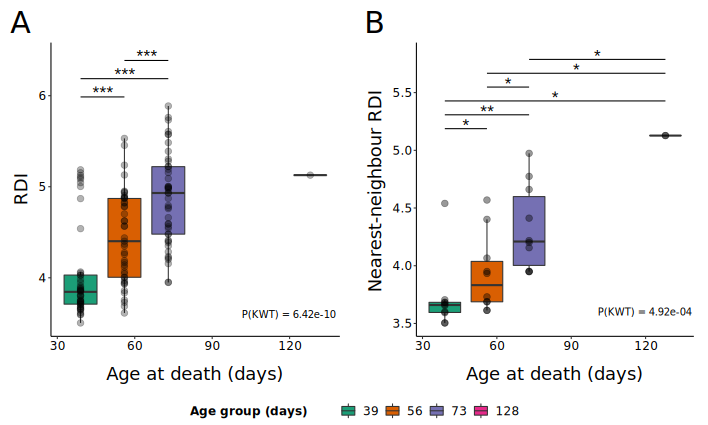
\includegraphics[width = 0.9\textwidth]{_Figures/png/ageing-rdi-VJ-individual-groupdist}
\begin{subfigure}{0em}
\phantomsubcaption{}
\label{fig:igseq-ageing-rdi-VJ-individual-groupdist-all}
\end{subfigure}
\begin{subfigure}{0em}
\phantomsubcaption{}
\label{fig:igseq-ageing-rdi-VJ-individual-groupdist-nn}
\end{subfigure}
\caption{Boxplots of overall (A) and nearest-neighbour (B) inter-individual VJ-RDI distances for each age group in the \igseq ageing dataset. Pairwise $p$-values are computed using nonparametric Mann–Whitney U tests ($*: 0.01 < p \leq 0.05;~**: 0.001 < p \leq 0.01;~***: p \leq 0.001$). $P(KWT)$ indicates the $p$-value of a Kruskal-Wallis analysis of variance test for a difference in RDI distribution with age.}
\label{fig:igseq-ageing-rdi-VJ-individual-groupdist}
\end{figure}

\begin{figure}
\centering
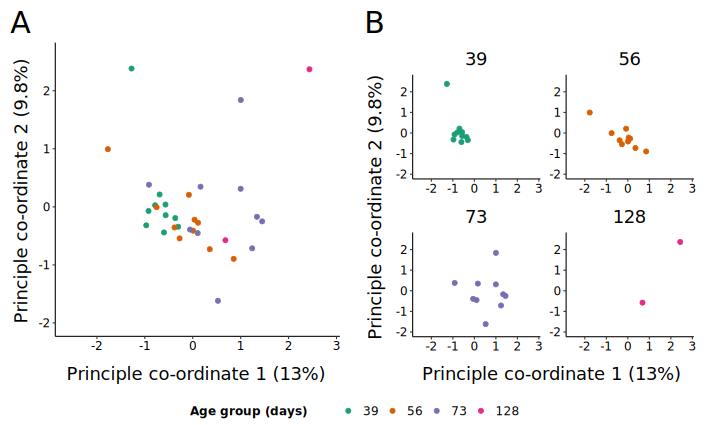
\includegraphics[width = 0.9\textwidth]{_Figures/png/ageing-rdi-VJ-individual-pcoa}
\begin{subfigure}{0em}
\phantomsubcaption{}
\label{fig:igseq-ageing-rdi-VJ-individual-pcoa-all}
\end{subfigure}
\begin{subfigure}{0em}
\phantomsubcaption{}
\label{fig:igseq-ageing-rdi-VJ-individual-pcoa-facet}
\end{subfigure}
\caption{Principal co-ordinate analysis (PCoA) of pairwise inter-individual VJ-RDI distances in the \igseq ageing dataset, coloured by age group and displayed together (A) or separately by age group (B).}
\label{fig:igseq-ageing-rdi-VJ-individual-pcoa}
\end{figure}


\clearpage\newpage
\section{Gut microbiota transfer and the turquoise killifish mucosal repertoire}
\label{sec:igseq_gut}

% TODO: Summarise ageing results, write segue

% TODO: Summary figure of gut microbiota study

Smith \textit{et al.} (2017) \parencite{smith2017microbiota} demonstrated that gut microbiota transfer from young to middle-aged turquoise killifish significantly extends lifespan in this species, as well as significantly altering microbiota composition and gene expression in the gut. As the gut microbiota in vertebrates is well-known to have an intimate relationship with the mucosal adaptive immune system, % TODO: Citation needed
it would be interesting to find out what effect microbiota transfer would have on the mucosal repertoires in turquoise killifish, and what if any relationship there is between these repertoires and the observed changes in microbiotal composition and lifespan. In particular, we hypothesised that gut microbiotal transfer might significantly ameliorate the ageing of the adaptive-immune repertoire seen in \Cref{sec:igseq_ageing}, either through delaying the decline in diversity observed in older fish or by stimulating a renewal of repertoire diversity in mucosal B-cells. In addition, by providing data on antibody repertoires of guts from young and old fish, such an experiment would provide a second, independent test of the effect of ageing on turquoise killifish repertoires, this time in a specific immune organ.

In order to investigate these questions, I designed an additional \igseq experiment in the turquoise killifish, using gut total RNA samples already available from the original microbiota-transfer study \parencite{smith2017microbiota}. 
As part of this study, total RNA was extracted from the isolated guts of twenty male turquoise killifish of the GRZ-Bellemans substrain (a closely-related substrain to the GRZ-AD substrain used in \Cref{sec:igseq_ageing}). These twenty individuals (\Cref{tab:gut-cohorts-summary,tab:gut-cohorts-fish}) were divided into two age cohorts and five treatment groups, with four untreated six-week-old fish (YI\_6wk) and sixteen sixteen-week-old fish in various treatment classes. Of the sixteen-week-old fish, four had undergone no treatment (WT\_16wk), four had undergone antibiotics treatment at nine weeks of age but no microbiota transfer (ABX\_16wk), four had undergone antibiotics treatment followed by microbiota transfer from a young (six-week-old) fish (YMT\_16wk) and the remaining four had received antibiotics at nine weeks of age followed by micriobiota transfer from a fish of the same age (OMT\_16wk).

\begin{table}[b]
% latex table generated in R 3.5.2 by xtable 1.8-3 package
% Fri Feb 22 10:04:14 2019
\begin{tabular}{lrlll}
  \toprule Group & Age (weeks) & \# Fish (Sequenced/Total) & Antibiotics? & Microbiota Transfer? \\ 
  \midrule YI\_6wk & 6 & 4 / 4 & No & No \\ 
  WT\_16wk & 16 & 3 / 4 & No & No \\ 
  ABX\_16wk & 16 & 4 / 4 & Yes & No \\ 
  SMT\_16wk & 16 & 3 / 4 & Yes & Yes (9-week-old donor) \\ 
  YMT\_16wk & 16 & 4 / 4 & Yes & Yes (6-week-old donor) \\ 
   \bottomrule \end{tabular}

\caption{Summary of killifish used in \igseq validation and ageing experiment. All fish are GRZ-Bellemans strain and male.}
\label{tab:gut-cohorts-summary}
\end{table}

Of these twenty samples, one (fish 400, from the WT\_16wk group) contained too little RNA to undergo \igseq library preparation, while another (fish 1005, from the OMT\_16wk group) was too degraded for a useful library to be obtained. The remaining 18 samples underwent \igseq library preparation, performed by Aleksandra Placzek and Michael Poeschla using the protocol I designed in \Cref{sec:igseq_protocol_library}. Several of the other samples were also somewhat degraded, with RNA integrity numbers between 5.5 and 7.0, but succeeded in producing useable libraries; these samples were included in the sequencing pool, but the RIN values from each sample were retained for comparison with downstream quality-control measures following \Igseq.

The libraries were sequenced together in two MiSeq runs, yielding a total of \embed{_Figures/txt/ageing-reads-raw-total.txt} million read pairs (\embed{_Figures/txt/gut-reads-raw-min.txt} to \embed{_Figures/txt/gut-reads-raw-max.txt} million pairs per individual), and the resulting reads underwent pre-processing, filtering and clonotyping as described in \Cref{sec:igseq_pilot,sec:igseq_ageing}. Compared to the datasets in those sections, the gut dataset exhibited highly consistent behaviour up to and including VDJ assignment and Change-O database construction, with \embed{_Figures/txt/gut-read-survival-init-min.txt}\,\% to \embed{_Figures/txt/gut-read-survival-init-max.txt}\,\% of reads surviving up to this stage in the pipeline (\Cref{fig:igseq-gut-read-survival-all}). However, a substantially higher proportion of reads (\embed{_Figures/txt/gut-read-survival-rel-loss-total.txt}\,\%) are lost during V-score filtering (\Cref{fig:igseq-gut-functional-prop}) and clonotyping, with some individuals losing as much as \embed{_Figures/txt/gut-read-survival-rel-loss-max.txt}\,\% of their input reads during these stages. The amount of reads lost at this stage did not appear to have any relationship with the RNA integrity of the samples (\Cref{fig:igseq-gut-read-survival-all-rin}, $r \approx -0.1$, $p \approx 0.7$).

To avoid any problems associated with very low numbers (and possibly low quality) of input reads, individuals with fewer than 30\% of input reads surviving through filtering and clonotyping were excluded from downstream analysis; two individuals (1274 and 1309, both from the antibotics-treated group) were excluded in this way (\Cref{fig:igseq-gut-read-survival-all-rel}).

\begin{figure}
\centering
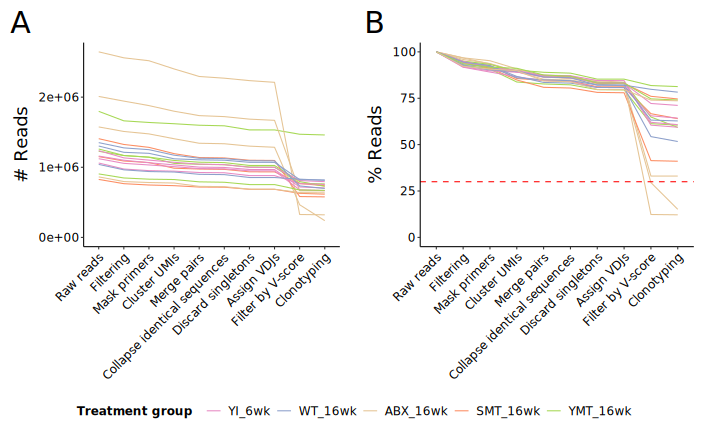
\includegraphics[width = 0.9\textwidth]{_Figures/png/gut-read-survival-all.png}
\begin{subfigure}{0em}
\phantomsubcaption{}
\label{fig:igseq-gut-read-survival-all-abs}
\end{subfigure}
\begin{subfigure}{0em}
\phantomsubcaption{}
\label{fig:igseq-gut-read-survival-all-rel}
\end{subfigure}
\caption{Absolute (A) and relative (B) read survival during pre-processing of the \igseq gut-microbiota-transfer dataset, up to and including clonotyping. The dotted red line in (B) indicates the 30\% read-survival cutoff, below which samples are discarded prior to downstream analysis.}
\label{fig:igseq-gut-read-survival-all}
\end{figure}

\begin{figure}
\centering
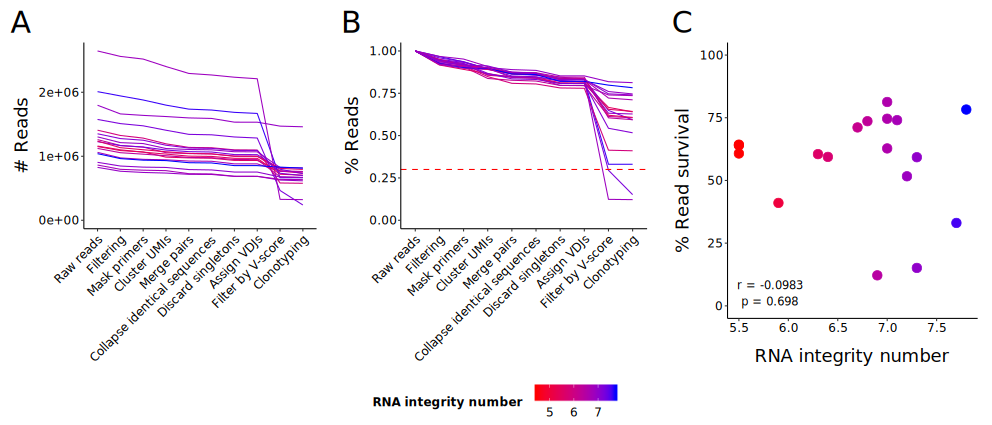
\includegraphics[width = \textwidth]{_Figures/png/gut-read-survival-all-rin.png}
\begin{subfigure}{0em}
\phantomsubcaption{}
\label{fig:igseq-gut-read-survival-all-rin-abs}
\end{subfigure}
\begin{subfigure}{0em}
\phantomsubcaption{}
\label{fig:igseq-gut-read-survival-all-rin-rel}
\end{subfigure}
\begin{subfigure}{0em}
\phantomsubcaption{}
\label{fig:igseq-gut-read-survival-all-rin-scatter}
\end{subfigure}
\caption[Relationship between RNA integrity and read survival in the gut \igseq dataset]{\textbf{Relationship between RNA integrity and read survival in the gut \igseq dataset:} (A-B) Absolute (A) and relative (B) read survival during pre-processing of the \igseq gut-microbiota-transfer dataset, up to and including clonotyping, coloured by the RNA integrity number of each input sample. The dotted red line in (B) indicates the 30\% read-survival cutoff, below which samples are discarded prior to downstream analysis. (C) Scatterplot of RNA integrity number \textit{versus} percentage read survival, up to and including clonotyping.}
\label{fig:igseq-gut-read-survival-all-rin}
\end{figure}


\begin{figure}
\centering
\includegraphics[width = 0.9\textwidth]{_Figures/png/gut-functional-prop}
\begin{subfigure}{0em}
\phantomsubcaption{}
\label{fig:igseq-gut-functional-prop-pre}
\end{subfigure}
\begin{subfigure}{0em}
\phantomsubcaption{}
\label{fig:igseq-gut-functional-prop-post}
\end{subfigure}
\caption{Proportion of input reads, UMI groups and unique sequences in the \igseq gut-microbiota-transfer dataset belonging to different (non)functional categories, before (A) and after (B) filtering on V-alignment score.}
\label{fig:igseq-gut-functional-prop}
\end{figure}

With two exceptions, the remaining samples from the gut microbiota transfer dataset exhibited a dramatically lower apparent clonal richness than either the pilot or ageing dataset, both in absolute terms (\Cref{fig:igseq-comparative-metrics-abs} -- with a median of \embed{_Figures/txt/igseq-gut-nclones-individual-med.txt} clones per individual compared to \embed{_Figures/txt/pilot-nclones-individual-med.txt} for the pilot dataset or \embed{_Figures/txt/ageing-nclones-individual-med.txt} for the ageing dataset) and relative to the number of UMI groups or unique sequences in each repertoire (\Cref{fig:igseq-comparative-metrics-rel}). This suggests, not entirely surprisingly, that killifish guts contain many fewer clones than whole-body killifish samples. However, the metrics presented in \Cref{fig:igseq-comparative-metrics} are strongly dependent on the size of each dataset: for example, even though the pilot dataset contains a subset of the individuals from the ageing dataset, their distributions in \Cref{fig:igseq-comparative-metrics} do not overlap.

In order to determine whether the apparent difference in clonal richness between the gut and other datasets is real, therefore, I performed rarefaction analysis, measuring the number of clones in repeated downsamplings of UMI groups from each dataset, along with the P20. % TODO: Already explained P20 above?
The results for the rarefied clonal counts (\Cref{fig:igseq-rarefied-clone-counts}) confirm the results from \Cref{fig:igseq-comparative-metrics-abs}: at any given downsampling size, the great majority of repertoires from the gut dataset contain far fewer clones than the repertoires in the pilot or ageing datasets. Concordantly, the gut repertoires also show a much greater degree of dominance by the largest clones in each repertoire, with over 85\% of gut samples exhibiting greater asymptotic P20 than over 90\% of ageing or pilot individuals and over 65\% exhibiting higher asymptotic P20 than any sample in the other experiments. In both cases (clonal counts and P20), a small minority of individuals deviate strongly from the general trend, exhibiting clonal counts and P20 values more consistent with those seen in the pilot and ageing experiments; however, only one individual (1412, from the 6-week-old untreated group) is an outlier in both clonal count and P20 value.

\begin{figure}
\centering
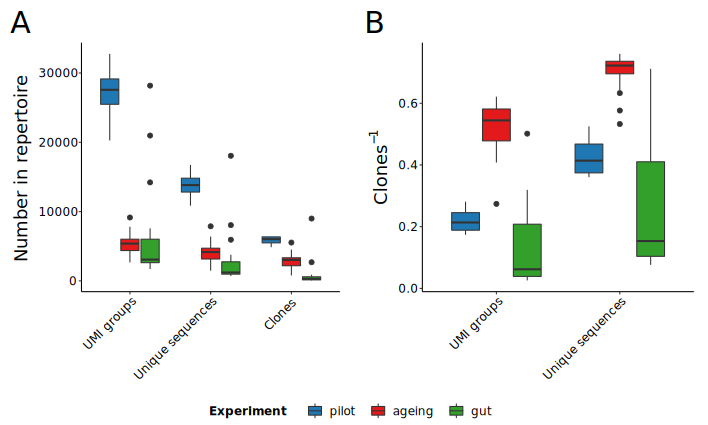
\includegraphics[width = 0.9\textwidth]{_Figures/png/igseq-comparative-metrics}
\begin{subfigure}{0em}
\phantomsubcaption{}
\label{fig:igseq-comparative-metrics-abs}
\end{subfigure}
\begin{subfigure}{0em}
\phantomsubcaption{}
\label{fig:igseq-comparative-metrics-rel}
\end{subfigure}
\caption{Absolute (A) and relative (B) read survival during pre-processing of the \igseq gut-microbiota-transfer dataset, up to and including clonotyping. The dotted red line in (B) indicates the 30\% read-survival cutoff, below which samples are discarded prior to downstream analysis.}
\label{fig:igseq-comparative-metrics}
\end{figure}

\begin{figure}
\centering
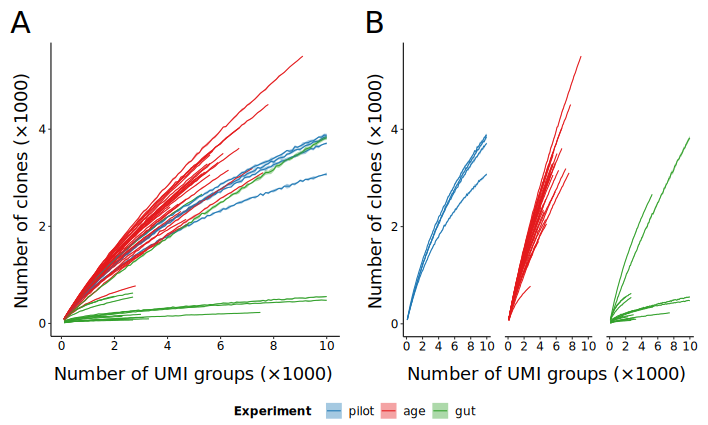
\includegraphics[width = 0.9\textwidth]{_Figures/png/igseq-rarefied-clone-counts}
\begin{subfigure}{0em}
\phantomsubcaption{}
\label{fig:igseq-rarefied-clone-counts-all}
\end{subfigure}
\begin{subfigure}{0em}
\phantomsubcaption{}
\label{fig:igseq-rarefied-clone-counts-facets}
\end{subfigure}
\caption{Rarefaction analysis of clonal counts in turquoise killifish repertoires from the \igseq pilot, ageing and gut-microbiota-transfer experiments, displayed together (B) and separately by experiment (B). Lines and shaded regions indicate the mean and standard deviation, respectively, over five replicates per sample size.}
\label{fig:igseq-rarefied-clone-counts}
\end{figure}
% TODO: Increase number of iterations (20?)

\begin{figure}
\centering
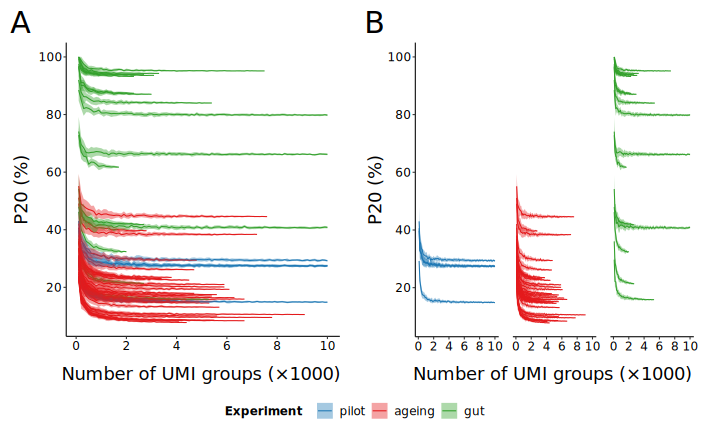
\includegraphics[width = 0.9\textwidth]{_Figures/png/igseq-rarefied-clone-p20}
\begin{subfigure}{0em}
\phantomsubcaption{}
\label{fig:igseq-rarefied-clone-p20-all}
\end{subfigure}
\begin{subfigure}{0em}
\phantomsubcaption{}
\label{fig:igseq-rarefied-clone-p20-facets}
\end{subfigure}
\caption{Rarefaction analysis of the proportion of each turquoise killifish repertoire occupied by the twenty largest clones (P20) in the \igseq pilot, ageing and gut-microbiota-transfer experiments, displayed together (A) and separately by experiment (B). Lines and shaded regions indicate the mean and standard deviation, respectively, over five replicates per sample size.}
\label{fig:igseq-rarefied-clone-p20}
\end{figure}
% TODO: Increase number of iterations (20?)

The killifish gut repertoire therefore exhibits not only a much lower clonal richness than the whole-body repertoire, but also in most cases a much greater degree of domination by the largest few clones. As briefly observed above, this is not altogether surprising: the whole-body repertoire includes clones from primary haematopoietic organs like the head kidney, which would be expected to contain many more small, \naive clones than a secondary lymphoid organ like the gut. In addition, as the B-cells in the gut are in close proximity and interaction with the gut microbiota, it is not surprising that they should show a much greater degree of clonal expansion and hence a larger average P20. Nevertheless, it is useful to confirm these phenomena, both as a sanity check about the quality of these datasets and because it may have important implications for the results of downstream analyses of the gut dataset.

% TODO: Zipf parameters? Other clonal measures?

The clonal alpha-diversity spectra for the gut dataset are shown in \Cref{fig:igseq-gut-clone-diversity-alpha}. At all diversity orders, there is a clear and drastic difference between the young (6-week-old) and old (16-week-old) groups, while the different 16-week-old treatment groups do not appear to show a strong difference in diversity. These observations are confirmed by statistical comparison of the distributions of individual diversity measurements at different diversity orders, which indicate highly significant differences in clonal repertoire diversity between young and old guts across the diversity spectrum (\Cref{fig:igseq-gut-clone-diversity-solo-age}), but no difference between treatment groups (\Cref{fig:igseq-gut-clone-diversity-solo-groups}). A similar pattern is observed for V/J-usage diversity (\Cref{fig:igseq-gut-VJ-diversity-alpha}), with a large and significant difference between young and old cohorts at many different diversity orders (\Cref{fig:igseq-gut-VJ-diversity-solo-age}) but no significant differences between 16-week-old treatment groups (\Cref{fig:igseq-gut-VJ-diversity-solo-groups}).

In terms of beta-diversity, the Hill-spectrum results (\Cref{fig:igseq-gut-VJ-diversity-beta}) are equivocal, with large differences in diversity between age groups observed at intermediate diversity orders (c. 1 to 2.5) but not at very low or very high orders (\Cref{fig:igseq-gut-VJ-diversity-beta-age}). Different treatment groups, meanwhile, exhibit very different patterns of beta diversity at higher orders (\Cref{fig:igseq-gut-VJ-diversity-beta-groups}), but not in any clear pattern: the antibiotic-treated and same-age-transfer groups show very high high-order beta diversity, indicating nearly maximal difference between individuals in their VJ-usage profiles, while the untreated and same-age-transfer groups show much lower between-individual variablity. To more closely investigate differences in inter-individual variability between sample groups, I again computed repertoire dissimilarity index (RDI) distances between each pair of individual repertoires in the dataset, and visualised the results by age cohort (\Cref{fig:igseq-gut-rdi-VJ-individual-age}) and treatment group (\Cref{fig:igseq-gut-rdi-VJ-individual-group}). The results again indicate large differences in VJ-usage variability between young and old gut repertoires in the turquoise killifish, with young samples clustering much more closely together (\Cref{fig:igseq-gut-rdi-VJ-individual-age-pcoa-facet}) and exhibiting consequently much lower pairwise RDI distances (\Cref{fig:igseq-gut-rdi-VJ-individual-age-groupdist-all,fig:igseq-gut-rdi-VJ-individual-age-groupdist-nn}); conversely, there is no significant difference in RDI distribution between the different 16-week-old treatment groups, indicating that the different groups are similar in their inter-individual variability. These RDI results contrast markedly with the differences in beta-spectra observed in \Cref{fig:igseq-gut-VJ-diversity-beta-groups}, suggesting that the latter may not be reliable measures of significant differences in intra-group variablity when sample sizes are small.

\begin{figure}
\centering
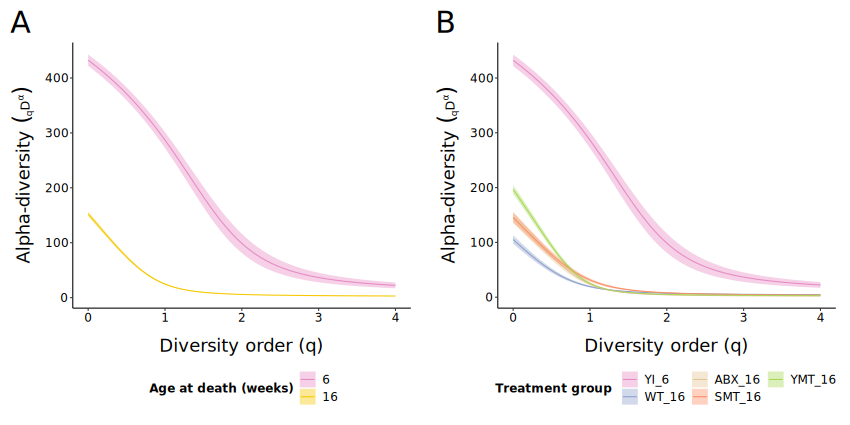
\includegraphics[width = 0.9\textwidth]{_Figures/png/igseq-gut-clone-diversity-alpha}
\begin{subfigure}{0em}
\phantomsubcaption{}
\label{fig:igseq-gut-clone-diversity-alpha-age}
\end{subfigure}
\begin{subfigure}{0em}
\phantomsubcaption{}
\label{fig:igseq-gut-clone-diversity-alpha-groups}
\end{subfigure}
\caption{Bootstrapped alpha-diversity spectra of clone sizes for each age (A) age group and (B) treatment group in the \igseq gut dataset, as measured by number of unique sequences per clone.}
\label{fig:igseq-gut-clone-diversity-alpha}
\end{figure}

\begin{figure}
\centering
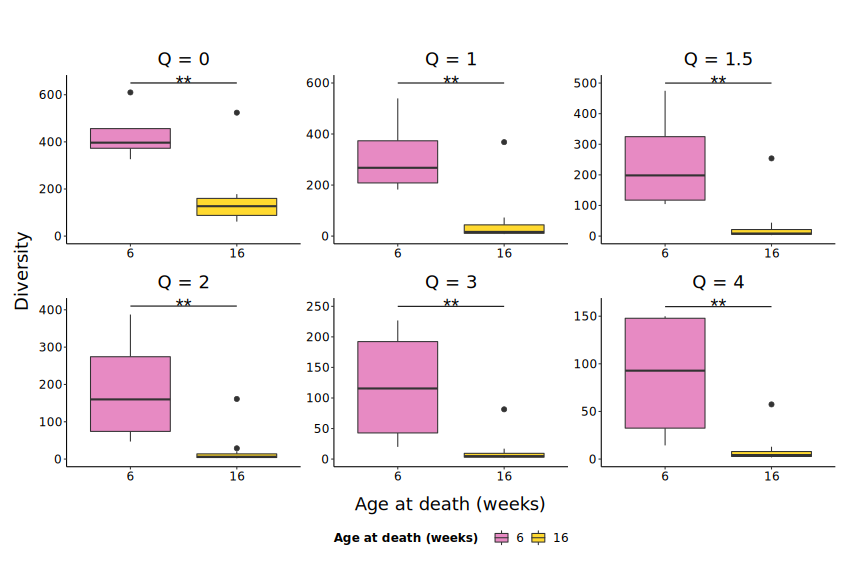
\includegraphics[width = 0.9\textwidth]{_Figures/png/igseq-gut-clone-diversity-solo-age}
\caption{Boxplots of \textit{clonal} Hill diversity values for the antibody repertoires of individuals of each age group in the \igseq gut dataset at a sample of diversity orders. Pairwise $p$-values are computed using nonparametric Mann–Whitney U tests ($*: 0.01 < p \leq 0.05;~**: 0.001 < p \leq 0.01;~***: p \leq 0.001$).}
\label{fig:igseq-gut-clone-diversity-solo-age}
\end{figure}

\begin{figure}
\centering
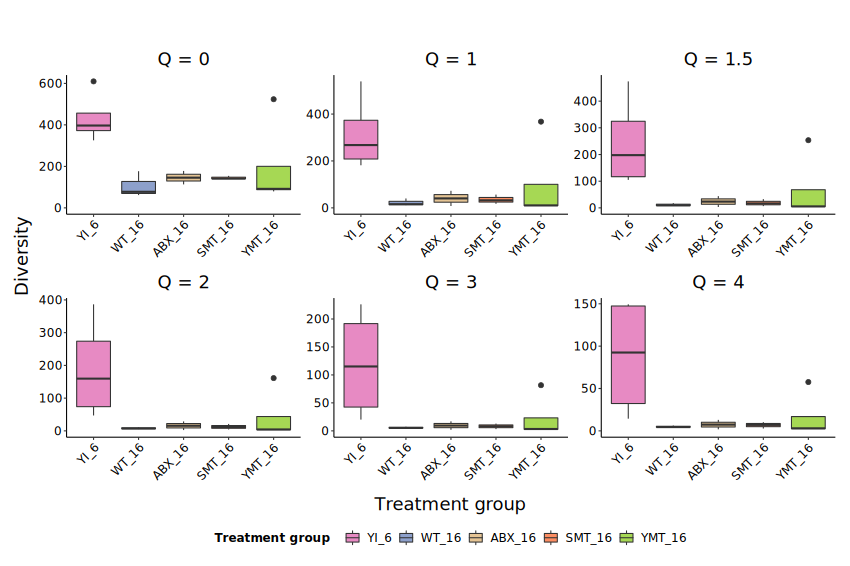
\includegraphics[width = 0.9\textwidth]{_Figures/png/igseq-gut-clone-diversity-solo-groups}
\caption{Boxplots of \textit{clonal} Hill diversity values for the antibody repertoires of individuals of each treatment group in the \igseq gut dataset at a sample of diversity orders. Pairwise $p$-values are computed using nonparametric Mann–Whitney U tests ($*: 0.01 < p \leq 0.05;~**: 0.001 < p \leq 0.01;~***: p \leq 0.001$).}
\label{fig:igseq-gut-clone-diversity-solo-groups}
\end{figure}

\begin{figure}
\centering
\includegraphics[width = 0.9\textwidth]{_Figures/png/igseq-gut-VJ-diversity-alpha}
\begin{subfigure}{0em}
\phantomsubcaption{}
\label{fig:igseq-gut-VJ-diversity-alpha-age}
\end{subfigure}
\begin{subfigure}{0em}
\phantomsubcaption{}
\label{fig:igseq-gut-VJ-diversity-alpha-groups}
\end{subfigure}
\caption{Bootstrapped alpha-diversity spectra of VJ usage for each (A) age group and (B) treatment group in the \igseq gut dataset, as measured by number of unique sequences per unambiguous VJ identity.}
\label{fig:igseq-gut-VJ-diversity-alpha}
\end{figure}

\begin{figure}
\centering
\includegraphics[width = 0.9\textwidth]{_Figures/png/igseq-gut-VJ-diversity-solo-age}
\caption{Boxplots of \textit{VJ} Hill diversity values for the antibody repertoires of individuals of each age group in the \igseq gut dataset at a sample of diversity orders. Pairwise $p$-values are computed using nonparametric Mann–Whitney U tests ($*: 0.01 < p \leq 0.05;~**: 0.001 < p \leq 0.01;~***: p \leq 0.001$).}
\label{fig:igseq-gut-VJ-diversity-solo-age}
\end{figure}

\begin{figure}
\centering
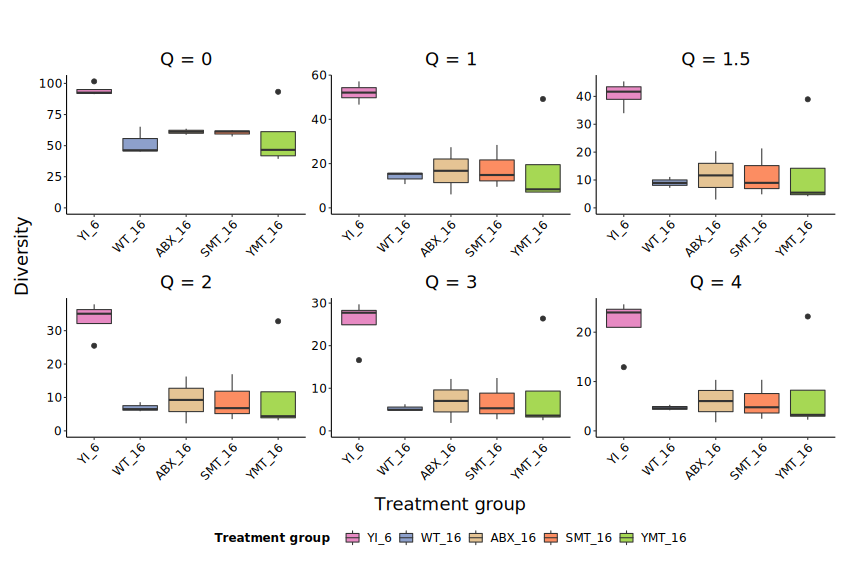
\includegraphics[width = 0.9\textwidth]{_Figures/png/igseq-gut-VJ-diversity-solo-groups}
\caption{Boxplots of \textit{VJ} Hill diversity values for the antibody repertoires of individuals of each treatment group in the \igseq gut dataset at a sample of diversity orders. Pairwise $p$-values are computed using nonparametric Mann–Whitney U tests ($*: 0.01 < p \leq 0.05;~**: 0.001 < p \leq 0.01;~***: p \leq 0.001$).}
\label{fig:igseq-gut-VJ-diversity-solo-groups}
\end{figure}

\begin{figure}
\centering
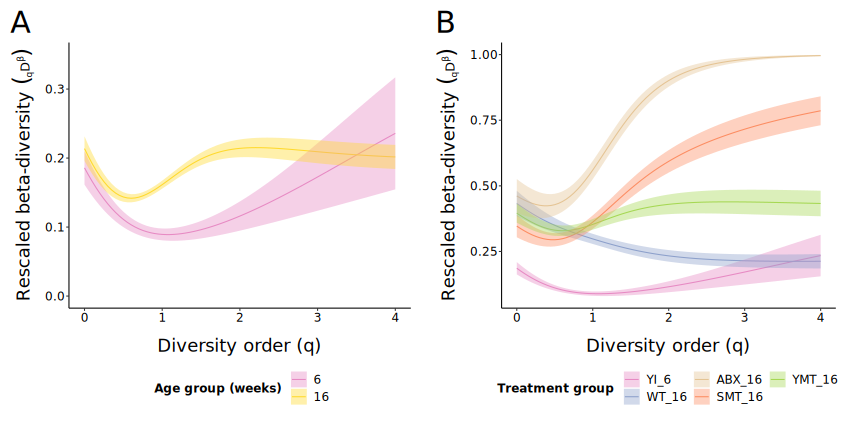
\includegraphics[width = 0.9\textwidth]{_Figures/png/igseq-gut-VJ-diversity-beta}
\begin{subfigure}{0em}
\phantomsubcaption{}
\label{fig:igseq-gut-VJ-diversity-beta-age}
\end{subfigure}
\begin{subfigure}{0em}
\phantomsubcaption{}
\label{fig:igseq-gut-VJ-diversity-beta-groups}
\end{subfigure}
\caption{Bootstrapped beta-diversity spectra of VJ usage, rescaled to between 0 (minimum) and 1 (maximum) for each (A) age group and (B) treatment group in the \igseq gut dataset.}
\label{fig:igseq-gut-VJ-diversity-beta}
\end{figure}


\begin{figure}
\centering
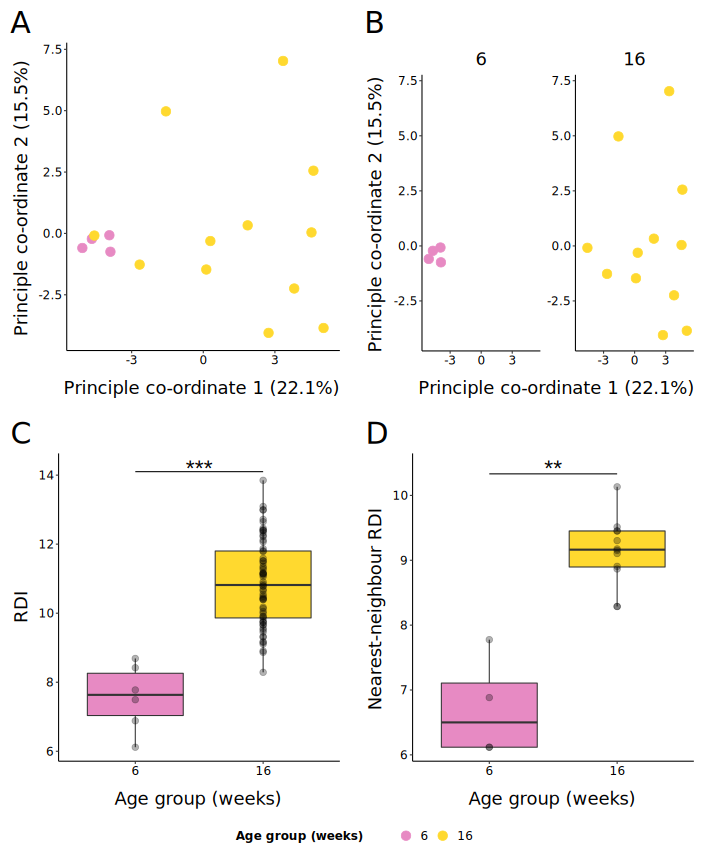
\includegraphics[width = 0.9\textwidth]{_Figures/png/igseq-gut-rdi-VJ-individual-age}
\begin{subfigure}{0em}
\phantomsubcaption{}
\label{fig:igseq-gut-rdi-VJ-individual-age-pcoa-all}
\end{subfigure}
\begin{subfigure}{0em}
\phantomsubcaption{}
\label{fig:igseq-gut-rdi-VJ-individual-age-pcoa-facet}
\end{subfigure}
\begin{subfigure}{0em}
\phantomsubcaption{}
\label{fig:igseq-gut-rdi-VJ-individual-age-groupdist-all}
\end{subfigure}
\begin{subfigure}{0em}
\phantomsubcaption{}
\label{fig:igseq-gut-rdi-VJ-individual-age-groupdist-nn}
\end{subfigure}
\caption{Intra-age-group variability in VJ expression in the \igseq gut dataset. (A-B) Principal co-ordinate analysis (PCoA) of pairwise inter-individual VJ-RDI distances, coloured by age group and displayed together (A) or separately by age group (B). (C-D) Boxplots of overall (C) and nearest-neighbour (D) inter-individual VJ-RDI distances for each age group in the dataset. Pairwise $p$-values are computed using nonparametric Mann–Whitney U tests ($*: 0.01 < p \leq 0.05;~**: 0.001 < p \leq 0.01;~***: p \leq 0.001$).}
\label{fig:igseq-gut-rdi-VJ-individual-age}
\end{figure}

\begin{figure}
\centering
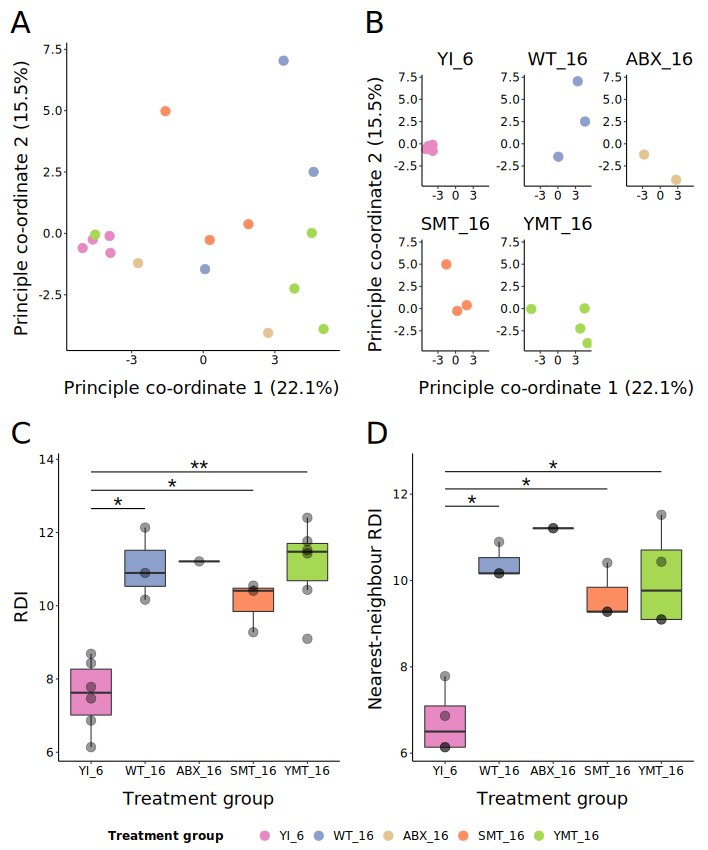
\includegraphics[width = 0.9\textwidth]{_Figures/png/igseq-gut-rdi-VJ-individual-group}
\begin{subfigure}{0em}
\phantomsubcaption{}
\label{fig:igseq-gut-rdi-VJ-individual-group-pcoa-all}
\end{subfigure}
\begin{subfigure}{0em}
\phantomsubcaption{}
\label{fig:igseq-gut-rdi-VJ-individual-group-pcoa-facet}
\end{subfigure}
\begin{subfigure}{0em}
\phantomsubcaption{}
\label{fig:igseq-gut-rdi-VJ-individual-group-groupdist-all}
\end{subfigure}
\begin{subfigure}{0em}
\phantomsubcaption{}
\label{fig:igseq-gut-rdi-VJ-individual-group-groupdist-nn}
\end{subfigure}
\caption{Intra-treatment-group variability in VJ expression in the \igseq gut dataset. (A-B) Principal co-ordinate analysis (PCoA) of pairwise inter-individual VJ-RDI distances, coloured by treatment group and displayed together (A) or separately by treatment group (B). (C-D) Boxplots of overall (C) and nearest-neighbour (D) inter-individual VJ-RDI distances for each treatment group in the dataset. Pairwise $p$-values are computed using nonparametric Mann–Whitney U tests ($*: 0.01 < p \leq 0.05;~**: 0.001 < p \leq 0.01;~***: p \leq 0.001$).}
\label{fig:igseq-gut-rdi-VJ-individual-group}
\end{figure}

These results strongly confirm the changes in killifish repertoire diversity with age observed in section \Cref{sec:igseq_ageing}, with older fish exhibiting a dramatic fall in alpha-diversity and increase in beta-diversity compared to young individuals. The results here are in fact even stronger than those from the whole-body ageing dataset, as there no significant result in VJ alpha-diversity was observed between age groups, while here both VJ and clonal alpha-diversity exhibit a strong and significant decline with age. This difference may result from the lower clonal richness and greater degree of oligoclonality exhibited in gut repertoires: when the local repertoire contains fewer small \naive clones and exhibits a greater degree of domination by the few largest clones, differences in VJ-usage between these large, activated clones may outweigh similar usage distributions in small, \naive clones to a greater extent than in the (much more polyclonal) whole-body repertoire.

% IGOR models: any change in generative distribution with age/treatment?

Conversely, there is no strong evidence from these analyses supporting the hypothesis that gut-microbiota transfer from young fish rejuvenates the antibody repertoire. While the alpha-diversity spectrum of the YMT group appears to be slightly higher than the OMT/ABX groups at very low diversity orders (\Cref{fig:igseq-gut-clone-diversity-alpha-groups}), these indications are not borne out by subsequent statistical analysis, and it is precisely these low-order diversity metrics that are most vulnerable to sampling bias and undersampling (a pervasive problem in \igseq). There is also no obvious difference in VJ alpha-diversity between treatment groups, while the beta-diversity of the YMT group is non-significantly \textit{higher} than that of the untreated control group (\Cref{igseq-gut-VJ-diversity-beta-groups,fig:igseq-gut-rdi-VJ-individual-group-groupdist-all}). Overall, whatever mechanism underlies the effect of gut microbiota transfer on killifish lifespan, it does not appear to be operating through modulation of gut antibody-repertoire diversity. 

\afterpage{%
    \begin{landscape}
        \centering
        \vspace*{\fill}
        \scriptsize
		% latex table generated in R 3.5.2 by xtable 1.8-3 package
% Fri Feb 22 10:04:13 2019
\begin{tabular}{llllll}
  \toprule Fish ID & Age at death (weeks) & Treatment group & Date of library prep & Sequenced? & Reason for exclusion \\ 
  \midrule 1271 & 16 & ABX\_16wk & 2018-11-20 & Yes & -- \\ 
  1274 & 16 & ABX\_16wk & 2018-12-01 & Yes & -- \\ 
  1309 & 16 & ABX\_16wk & 2018-12-01 & Yes & -- \\ 
  dash & 16 & ABX\_16wk & 2018-12-01 & Yes & -- \\ 
  1015 & 16 & SMT\_16wk & 2018-11-20 & Yes & -- \\ 
  1298 & 16 & SMT\_16wk & 2018-11-20 & Yes & -- \\ 
  1301 & 16 & SMT\_16wk & 2018-11-20 & Yes & -- \\ 
  402 & 16 & WT\_16wk & 2018-11-20 & Yes & -- \\ 
  938 & 16 & WT\_16wk & 2018-11-20 & Yes & -- \\ 
  940 & 16 & WT\_16wk & 2018-11-20 & Yes & -- \\ 
  1403 &  6 & YI\_6wk & 2018-11-20 & Yes & -- \\ 
  1409 &  6 & YI\_6wk & 2018-12-01 & Yes & -- \\ 
  1412 &  6 & YI\_6wk & 2018-11-20 & Yes & -- \\ 
  1414 &  6 & YI\_6wk & 2018-11-20 & Yes & -- \\ 
  1009 & 16 & YMT\_16wk & 2018-11-20 & Yes & -- \\ 
  1026 & 16 & YMT\_16wk & 2018-11-20 & Yes & -- \\ 
  1305 & 16 & YMT\_16wk & 2018-11-20 & Yes & -- \\ 
  999 & 16 & YMT\_16wk & 2018-12-01 & Yes & -- \\ 
  400 & 16 & WT\_16wk & -- & No & Not enough RNA for library prep \\ 
  1005 & 16 & SMT\_16wk & -- & No & RNA integrity too low \\ 
   \bottomrule \end{tabular}

		\normalsize\vspace{1em}
        \captionof{table}{Turquoise killifish used in \igseq validation and ageing experiment. All fish are GRZ-Bellemans strain and male.}
        \label{tab:gut-cohorts-fish}
        \vspace*{\fill}
    \end{landscape}
}
% TODO: Try to get detailed information on cohorts (birth and death dates, age in days, etc.)